\documentclass[10pt,aps,onecolumn,notitlepage,nofootinbib]{revtex4-2}
\usepackage{amsmath,amssymb,mathtools,bm}
\usepackage{booktabs,array,graphicx,hyperref,microtype}
\hypersetup{hidelinks}
\newcommand{\vk}{\bm k}
\newcommand{\ve}{\bm e}
\newcommand{\vu}{\bm u}
\newcommand{\vf}{\bm f}
\newcommand{\vF}{\bm F}
\newcommand{\vR}{\bm R}
\newcommand{\veta}{\bm\eta}
\newcommand{\vchi}{\bm\chi}
\newcommand{\qT}{\mathrm{qT}}
\newcommand{\qL}{\mathrm{qL}}
\newcommand{\ImH}{\operatorname{Im}_{\!H}}
\newcommand{\order}{\mathcal O}
\newcommand{\Tr}{\operatorname{Tr}}
\ifdefined\pdftrailerid\pdftrailerid{}\fi
\renewcommand{\thesection}{SM\arabic{section}}
% Source identity and validation scope (comments only; no typeset content).
% Working edition: end matter following the approved Section IX, 11 November 2026.
% PACKAGE_SHA256SUMS.json records the files in this cumulative package.
% checks/BUILD_CHECK.json identifies the corresponding main and supplemental build.
% checks/IX_APPROVED_CLAIMS.json and checks/VIII_CERTIFICATES.json distinguish the
% original reference-taper certificate from the separate bounds for the increasing ramp.
% These scientific inputs and bounds are retained in the present editorial revision.
% The following comments are historical. Each edition label and hash refers to its own release.
% Current edition: checked corrections and prediction-evidence revision, 28 September 2026 (Toronto).
% Current source identities, applied edits and completed checks: checked_revision_manifest.json.
% Exact manuscript changes: checked_revision_edits.json (40 spans:17 main,23 supplement;39 reported plusC17 angular path).
% Main and supplement retain onecolumn. Historical numerical table entries are preserved.
% The branch-edge proof, local definitions, navigation and evidence wording follow the checked report.
% New and preceding check records are identified in EVIDENCE_ACCESS.md and evidence/.
% This source update does not enlarge the fixed-frequency R8 certificate.
% Original GB producer history and factual author/disclosure/public-release items remain bounded open matters.
% All previous source-binding text is preserved below as historical provenance.
% ---- Preserved preceding source-binding records follow ----
% Current edition: two-perspective framing revision, 27 September 2026 (Toronto).
% Current source identities and checks: two_perspective_framing_manifest.json.
% Exact changes: two_perspective_framing_edits.json (E1-E3, three main prose spans).
% Abstract and supplement unchanged; both documents retain onecolumn.
% No numerical recertification, new clock model, or enlargement of claim scope.
% All earlier source-binding text is preserved below as historical provenance.
% ---- Preserved preceding source-binding records follow ----
% Current edition: final referee revision, 27 September 2026 (America/Toronto).
% Current identities/checks: referee_revision_manifest.json.
% Exact manuscript replacements: referee_revision_edits.json (14 spans).
% Main and supplement remain single-column. No broad cuts or relocations.
% Selected display rounding and shell-estimate wording do not rerun or enlarge R8.
% Factual author/release/disclosure tasks remain open as stated in the report.
% All earlier records below describe their historical editions.
% ---- Preserved previous source-binding records follow ----
% Current revision: 27 September 2026, four contribution-clarity edits E1--E4.
% Current file identities and completed checks: contribution_clarity_revision_manifest.json.
% Exact manuscript replacements: contribution_clarity_edits.json (4 spans).
% Only main-paper prose changes; the supplement and scientific results are retained.
% This revision does not rerun or extend the R8 certificate.
% Earlier records below describe their own historical editions.
% ---- Preserved previous source-binding record follows ----
% Current revision: 27 September 2026, minimum current-issues corrections.
% Current file identities and completed checks: current_issue_revision_manifest.json.
% Exact manuscript replacements: current_issue_edits.json (10 spans).
% Earlier records below are historical, not identities of this revision.
% Both documents remain single-column; no scientific equations/results changed.
% This revision does not rerun or extend the R8 certificate.
% ---- Preserved earlier source-binding record follows ----
% Editorial shortening and clarity revision implemented, 27 September 2026.
% Current source hashes and all applied edit IDs are recorded in
% editorial_revision_manifest.json; editorial_edits.json supplies exact spans.
% This is a source/layout revision, not a new numerical validation or an
% extension of the R8 certificate. Scientific equations/results retain their
% stated evidence and scope. The comments below and the unchanged
% prediction_integration_manifest.json are historical baseline records.
% ---- Preserved prediction-integration and earlier provenance below ----
% Prediction-integrated manuscript build, 27 September 2026.
% The record below is retained baseline provenance, not a hash description
% or certification of the prediction-integrated sources. See the accompanying
% integration manifest for their current hashes and change record.
% R8 has not been rerun or expanded to certify these new predictions.
% ---- Preserved baseline provenance begins below ----
% Paper One source correspondence: focused revision, 26 September 2026.
% This file is intentionally comments only. It changes no typeset content.
% Compile from this directory: latexmk -pdf paper1_main.tex
% and: latexmk -pdf paper1_supplement.tex
% Alternatively, run pdflatex on each source until references stabilize.
% Both bibliographies are explicit; latexmkrc disables unnecessary BibTeX.
%
% Baseline: PAPER1_LATEX_BUILD_2026-09-26(2).zip.
% Supporting validation: PAPER1_VALIDATION_INTEGRATED_R8(1).zip.
% R8 and its validator are unchanged. Its exact-source check validates its
% archived manuscript/candidate, not these revised TeX files.
% This record associates unchanged mathematics/results with that evidence;
% hashes establish file identity, not a new numerical certification.
% All 185 original displayed math blocks and all eight original tables are
% retained byte-for-byte and in order. No original section or label is lost.
% Original figure data are retained. The selector receives styling changes;
% the additional spectrum displays the existing 49 ACTIVE85 frequency rows.
% The three new displayed formulas and continuum interference table explain
% or evaluate existing source and spectral constructions. Their scope is
% stated in main Secs. IV-VI and supplement SM4; they do not enlarge the
% certified frequency/coupling domain or assert a new continuum-limit proof.
% Main and supplement retain their conditional observer/clock explanations.
% Public archive citation and genuine author contact details remain pending
% as stated in the manuscript. No public deposit is implied by this record.
%
% SHA-256 of original attached sources:
% paper1_main.tex bb1a14bed6775ee6011643aa830cc7cc0c84a7418bc6a1b9c1314276eb8d2dc9
% paper1_supplement.tex bf687d7424050fefd9571072c1fbf4fb24db90690cdcdfd6b0ab85696fcc3786
% SHA-256 of R8 candidate sources:
% manuscript/candidate/paper1_main.tex b6e94ea9f60b27bb428085f1fb6a027bbfbdb0831d3fdcd13dae128fc97dc58f
% manuscript/candidate/paper1_supplement.tex d9b77cfbc9053b2087d1d06dd8032add3e72465ab890602da182d977a4c255a9
% Existing R8 input authority for the added spectrum:
% legacy_rc4/validation/current_numerics/analysis/resolution_execution/robustness/ACTIVE85.json
% sha256 93ae058159343720a54fb272b2d9f9dd5b0cce839d652bf1e0e66f69b8174ef5
% Additional diagnostic records from the reassessment (outside unchanged R8):
% continuum_weak_results.json 21ab02f827e73c22cd6ee8762f1535407202aa8881803730026a1e5496d56d3d
% weak_crosscheck_results.json 449e088b87df319244c27c852f7feaf519d39d52825d306a1a6feb6e5773e90e
% These new diagnostics are specified by the formulas, normalizations,
% source parameters, and quadrature ladders given in supplement SM4.
% They are not claimed to be pre-existing outputs of the R8 validator.
% SHA-256 of final build inputs, excluding this self-describing file:
% aps10pt4-2.rtx 0cc5d7fab6ffd59ba5779f9ddfad990cb8a71438ea390277bafff1824bbcb8e4
% aps4-2.rtx 52d33501cae6dfdf339efeb2a79fda0a2780d1d39d96b61a1c6a6311da6ca05e
% figures/Halpha_transmission_scan_p06.png 04948c9231a539082d234c3af2a68e7d10d560e42f9c6f2e51f589053235cb3d
% figures/continuum_lattice_share_comparison_p06.png e2323d751a32fdfb30f7c39acb5ab33d349e41b0f773cca8d3bd7f14d30e7e02
% figures/paper1_frequency_partition.pdf a446ec83b61e2b8c6c70c6f638c9e95d60ffa74b3b8967304ce45ce392636aa5
% figures/paper1_sectionIV_fig3_bulk_modes_symmetry_v2.pdf 9882955f2a34701f5154841c2325fff32d3344f619e7a1438d2a8672c56575b8
% figures/paper1_sectionVII_fig6a_qT_window_v2.pdf b5de298d32a530958519505a607765331a569cb3de6ef18c6a1e133c5be3836d
% figures/paper1_sectionVII_fig6b_selector_controls_v2.pdf 0d5cfcb0ad6f88ea1c6b4fc6c4cedc282acf52728af4ffc8f7ffe4216642411a
% figures/paper1_sectionVI_fig4_reference_partition_v2.pdf 7c5313c544de0373b3e234355c143d404ec3c569efcd946d7e477b47798f67c1
% latexmkrc abed4d537fbfeeac0ef306877b6a97528125588e4a2344f07e79cab771bc2b0c
% paper1_main.tex de18909953cd48e9828af791d7c755cdf63eefc84d3b6ce9c4d22151de3d36b0
% paper1_methods_references.tex e219c707377f6ed3c2c86cffd6a7cffc9f358cbcb9a334450dad7127de9b8d08
% paper1_supplement.tex e4cf3a1573c3583bab964eccb0e5b93b266aa635cd08926e766b10c9e47f6186
% revsymb4-2.sty 7614d7446d929f49917e54c8590d7ff7408572a9d2d293d209ea718540947d3e
% revtex4-2.cls 58727044fa47fff2663615774f8f24baab978944bbc55f84f8dc08ef91f67358

\begin{document}
\title{Supplementary material for Low-Frequency Radiation at a Reciprocal Junction between a Line and a Three-Dimensional Harmonic Lattice}
\author{Mike Fernandes}
\email[Corresponding author: ]{mike1fernand@gmail.com}
\affiliation{Independent Researcher, Ontario, Canada}
\maketitle

This supplement records the analytic regressions, singular-integration definitions, deterministic convergence checks, scalar-model robustness data, and coefficient-blind real-time controls used by the main text. Machine-readable records and producer code are provided in the validation archive described in the main paper's Data Availability Statement. Large real-space snapshot arrays are regenerated using the documented validation workflow rather than distributed in the compact archive. No result described here upgrades the discrete-lattice finite-coupling-region claim to a continuum, polarization-control, gauge, or electromagnetic theory.

Section~SM7 gives the additional prediction derivations and numerical checks, with their parameter domains and limits. These records are separate from the fixed-frequency tolerance bound for the reference contact in Sec.~SM5B.

Unless stated otherwise, we use equilibrium lattice coordinates, Hamiltonian time $\tau$ and the main text's mechanical energy convention. Frequencies, speeds, currents, snapshots and reporting intervals refer to this time, and overdots denote $d/d\tau$. Section~\ref{sec:sm-perspectives} distinguishes internal-observer descriptions and gives a conditional time-coordinate translation.

Where the finite reference device is indexed locally, $s=1,\ldots,N_c$ denotes global segment $i_0+s-1$, $g_s\equiv g_{i_0+s-1}$, and segment $s$ joins local line sites $q_{s-1}$ and $q_s$.

\section{Harmonic expansion, force identities, and finite source}

\paragraph*{Harmonic origin.}
For a bond family $\alpha$ with equilibrium vector $\bm d=r_{0,\alpha}\hat{\bm d}$, assume $V_\alpha\in C^3$ locally,
\begin{equation}
 V_\alpha'(r_{0,\alpha})=0,
 \qquad V_\alpha''(r_{0,\alpha})=\kappa_\alpha>0.
\end{equation}
For $|\Delta\vu|\ll r_{0,\alpha}$,
\begin{align}
 |\bm d+\Delta\vu|-r_{0,\alpha}
 &=\hat{\bm d}\cdot\Delta\vu
 +\frac{|\Delta\vu|^2-(\hat{\bm d}\cdot\Delta\vu)^2}{2r_{0,\alpha}}
 +\order(|\Delta\vu|^3/r_{0,\alpha}^2),\\
 V_\alpha(|\bm d+\Delta\vu|)-V_\alpha(r_{0,\alpha})
 &=\frac{\kappa_\alpha}{2}(\hat{\bm d}\cdot\Delta\vu)^2
 +\order(\Lambda_\alpha|\Delta\vu|^3).
\end{align}
The production model is the exact quadratic Hamiltonian defined by the retained term.  The line, axial-bulk, face-diagonal, and source-link rest lengths are $a$, $a$, $\sqrt2a$, and $\sqrt3a/2$, respectively.

\paragraph*{Source coordinates and optional inverse-spacing dictionary.}
For the main text's paired-link geometry, $c=(s_y,s_z)$ with $s_y,s_z=\pm1$. Define $\bm t_c=s_y\hat{\bm y}+s_z\hat{\bm z}$, so $|\bm t_c|=\sqrt2$, and
\begin{equation}
 \bar q_i=\frac{q_i+q_{i+1}}{2},\qquad
 \Delta q_i=q_{i+1}-q_i,\qquad
 S_{ic}=\bm t_c\cdot\vu_{ic}.
\end{equation}
The optional inverse-spacing dictionary is
\begin{equation}
\begin{gathered}
  \epsilon_i=\Delta q_i/a,
  \qquad 1+\epsilon_i>0,\\
  n_{q,i}=[a+\Delta q_i]^{-1},
  \qquad n_{q,\mathrm{ref}}=a^{-1},\\
  \frac{n_{q,i}}{n_{q,\mathrm{ref}}}
  =(1+\epsilon_i)^{-1}
  =1-\epsilon_i+\order(\epsilon_i^2).
\end{gathered}
\label{eq:sm-inverse-spacing}
\end{equation}
Positive $\Delta q_i$ means extension and negative $\Delta q_i$ means compression. The last equality is a small-strain expansion. Here $n_{q,i}$ is the reciprocal of the deformed line-segment length $a+\Delta q_i$. It specifies neither a three-dimensional background density nor a clock-rate law. This is only a kinematic interpretation: the forces in main Sec.~3 follow from the paired-link energy, with coordinates
\begin{equation}
 A_{ic}=u_{ic,x}-\bar q_i,
 \qquad
 B_{ic}=s_yu_{ic,y}+s_zu_{ic,z}+\frac{\Delta q_i}{2}.
\end{equation}
The two physical signed extensions obey
\begin{equation}
 e_L=\frac{A_{ic}+B_{ic}}{\sqrt3},
 \qquad
 e_R=\frac{B_{ic}-A_{ic}}{\sqrt3},
\end{equation}
so that
\begin{equation}
 \frac{g_i}{2}(e_L^2+e_R^2)=\frac{g_i}{3}(A_{ic}^2+B_{ic}^2),
 \quad
 H_{X,ic}=\frac{g_i}{4}(e_L-e_R)^2,
 \quad
 H_{R,ic}=\frac{g_i}{4}(e_L+e_R)^2.
\end{equation}
The complete coupling sectors are
\begin{equation}
 H_X=\sum_{i\in\mathcal I_c}\sum_{s_y,s_z=\pm1}H_{X,ic},
 \qquad
 H_R=\sum_{i\in\mathcal I_c}\sum_{s_y,s_z=\pm1}H_{R,ic},
 \qquad H_c=H_X+H_R.
\end{equation}
Symbolic differentiation reproduces all three corner-force components and both scalar endpoint generalized forces exactly. A randomized five-point force-gradient test gives a maximum scaled error below $4.21\times10^{-14}$.

\paragraph*{$X/R$ component powers and storage.}
For the source coordinates above, $X$ is the axial-average sector and $R$ is the segment-strain/radial sector. They are not bulk eigenbranch labels. The following identities supply the detailed local bookkeeping used in main Sec.~3.3. Define the powers done by the coupling force on the bulk and line subsystems,
\begin{align}
  P_{b,X}^{ic}&=-\frac{2g_i}{3}A_{ic}\dot u_{ic,x},
  &P_{q,X}^{ic}&=\frac{2g_i}{3}A_{ic}\dot{\bar q}_i,
  \label{eq:sm-X-powers}\\
  P_{b,R}^{ic}&=-\frac{2g_i}{3}B_{ic}\dot S_{ic},
  &P_{q,R}^{ic}&=-\frac{g_i}{3}B_{ic}\dot{\Delta q}_i.
  \label{eq:sm-R-powers}
\end{align}
Because $g_i$ is time independent,
\begin{equation}
  \dot H_{X,ic}=-(P_{b,X}^{ic}+P_{q,X}^{ic}),
  \qquad
  \dot H_{R,ic}=-(P_{b,R}^{ic}+P_{q,R}^{ic}).
  \label{eq:sm-local-work}
\end{equation}
Global interface powers are obtained by summing over $i\in\mathcal I_c$ and the four corners. The power delivered to the line and bulk need not be instantaneously equal and opposite because the coupling energy can store energy. Local work is exactly additive in $X$ and $R$; same-full-state field or flux interference and separately redressed sector controls, as distinguished in main Sec.~6.3, are different constructions.

\paragraph*{Finite fixtures and conditional kernel.}
For any declared finite truncation, collect the signed longitudinal bond extensions in a compatibility matrix $\mathsf B_{\rm comp}$ and the positive spring constants in a diagonal matrix $W$. Then
\begin{equation}
 K=\mathsf B_{\rm comp}^{\mathsf T}W\mathsf B_{\rm comp},
 \qquad
 \ker K=\ker\mathsf B_{\rm comp},
\end{equation}
which makes nonnegativity and exact extension-preserving zero modes explicit. Here the distinct symbol $\mathsf B_{\rm comp}$ avoids confusion with the local source coordinate $B_{ic}$.

Under the declared free-boundary and included-bond convention, representative bulk boxes of sizes $2\times2\times2$, $3\times2\times2$, $3\times3\times3$, and $4\times3\times3$ each have six rigid-body modes---three translations and three rotations. One- through four-segment combined line--bulk fixtures each have nullity two. If the finite bulk framework is infinitesimally rigid, the scalar line is connected, and at least one complete positive four-corner/eight-link source motif is present, the exact combined kernel is spanned by common axial translation and rigid bulk rotation about the line. Removing the source coupling restores the seven disconnected rigid/line modes. The complete coordinate ordering, included-bond convention, singular-value tolerance, fixture results, and mutation controls are provided in the validation archive.

\paragraph*{Source transforms and prescribed-Bloch asymptotics.}
This paragraph supplements the dressed finite-slab source in main Sec.~3.2. The line-driven radial source is
\begin{equation}
 \vf^{\rm src}_{R,ic}=-\frac{g_i}{3}\Delta q_i(s_y\hat{\bm y}+s_z\hat{\bm z}).
\end{equation}
With transverse corner radius $\bm r_c=(a/2)\bm t_c$, the four corners satisfy
\begin{equation}
 \sum_c\vf^{\rm src}_{R,ic}=0,
 \qquad
 \sum_c\bm r_c\times\vf^{\rm src}_{R,ic}=0,
 \qquad
 M^R=-\frac{2g_i a\Delta q_i}{3}\operatorname{diag}(0,1,1).
\end{equation}
The dipole is contractile for extension and extensile for compression.  The complete force/torque closure is restricted to the centered $C_{4v}/A_1$ sector; an off-symmetry negative control gives nonzero transverse endpoint reactions.

For the spatial Fourier convention $e^{-i\vk\cdot\bm r}$, the transverse four-corner source factor is
\begin{equation}
  \widetilde{\vF}^{\rm src}_{R,i}(k_y,k_z)
  =\frac{4ig_i\Delta q_i}{3}
  \begin{pmatrix}
    0\\
    \sin(k_ya/2)\cos(k_za/2)\\
    \cos(k_ya/2)\sin(k_za/2)
  \end{pmatrix}.
  \label{eq:sm-local-fourier}
\end{equation}
For a monochromatic state, the same expression uses the complex difference amplitude in place of $\Delta q_i$. For an arbitrary fixed-frequency dressed line state, write
\begin{equation}
 q_i(\tau)=\operatorname{Re}[Q_i^{\rm full}(\omega)e^{-i\omega\tau}],
 \qquad
 \bar Q_i^{\rm full}=\frac{Q_i^{\rm full}+Q_{i+1}^{\rm full}}{2},
 \qquad
 \Delta Q_i^{\rm full}=Q_{i+1}^{\rm full}-Q_i^{\rm full}.
\end{equation}
The full finite-slab radial-source transform is
\begin{align}
 \widetilde{\vf}^{\rm slab}_{R}(\vk;\omega)
 &=\frac{4i}{3}\bm s_\perp(\vk)
 \sum_{i\in\mathcal I_c}g_i\Delta Q_i^{\rm full}(\omega)
 e^{-ik_x(i+1/2)a},\\
 \bm s_\perp(\vk)&=
 \begin{pmatrix}
 0\\ \sin(k_ya/2)\cos(k_za/2)\\
 \cos(k_ya/2)\sin(k_za/2)
 \end{pmatrix}.
\end{align}
The axial-average source component is
\begin{equation}
 \widetilde{\vf}^{\rm slab}_{X}(\vk;\omega)
 =\frac{8}{3}\hat{\bm x}
 \cos(k_ya/2)\cos(k_za/2)
 \sum_{i\in\mathcal I_c}g_i\bar Q_i^{\rm full}(\omega)
 e^{-ik_x(i+1/2)a},
\end{equation}
and the complete line-driven source transform is
\begin{equation}
 \widetilde{\vf}^{\rm slab}_{X+R}
 =\widetilde{\vf}^{\rm slab}_{X}
 +\widetilde{\vf}^{\rm slab}_{R}.
\end{equation}
For the special pure Bloch component $Q_i=Qe^{i\kappa ia}$, the axial part reduces to
\begin{equation}
 \widetilde{\vf}^{\rm slab}_{X}(\vk;\kappa)
 =\frac{8Q}{3}\cos(\kappa a/2)\,
 \mathcal A(\kappa-k_x)
 \cos(k_ya/2)\cos(k_za/2)\hat{\bm x},
\end{equation}
while the radial part reduces to
\begin{align}
 \widetilde{\vf}^{\rm slab}_{R}(\vk;\kappa)
 &=-\frac{8Q}{3}\sin(\kappa a/2)\,
 \mathcal A(\kappa-k_x)\bm s_\perp(\vk),\\
 \mathcal A(\kappa-k_x)
 &=\sum_{i\in\mathcal I_c}g_i e^{i(\kappa-k_x)(i+1/2)a}.
\end{align}
For the same prescribed pure Bloch component, remove the segment-midpoint phase and take $\rho^2=\kappa^2+k_y^2+k_z^2$ with $\rho a\ll1$. At fixed $Q$, lattice spacing, coupling profile, and number of active segments,
\begin{equation}
 e^{-i\kappa(i+1/2)a}
 \widetilde{\vF}^{\rm src}_{R,i}
 =-\frac{2g_i a^2Q}{3}
  \begin{pmatrix}0\\ \kappa k_y\\ \kappa k_z\end{pmatrix}
 +\order(g_i|Q|a^4\rho^4).
 \label{eq:sm-long-wave-source}
\end{equation}
This local bare-source expansion is not the fixed-contact dressed low-frequency transmission law of main Sec.~5.3.

These pure-Bloch $X$ and $R$ components define the complete bare $X+R$ source used in the shell-overlap witnesses of SM2. A direct segment/corner sum with independently randomized $\kappa$ and $k_x$ agrees below $2\times10^{-14}$ scaled error. Because the radial-source resultant vanishes, its first moment controls the leading transverse-wave-number term,
\begin{equation}
 \widetilde{\vf}^{\rm src}_{R,i}(\vk_\perp)
 =-i\bm M_i^R\vk_\perp
 +\order(g_i|\Delta q_i|a^3|\vk_\perp|^3).
\end{equation}
Moreover,
\begin{equation}
 \|\bm s_\perp(\vk)\|^2
 =\frac{1-\cos(k_ya)\cos(k_za)}{2},
\end{equation}
Because this factor is independent of $k_x$, its exact nodal set in the closed transverse first Brillouin zone consists of the full axial line $(k_y,k_z)=(0,0)$ and the periodically identified axial lines through the transverse zone corners $(k_y,k_z)=(\pm\pi/a,\pm\pi/a)$, for every allowed $k_x$. After removing the segment-midpoint phase, the leading radial-source amplitude has order two and the post-leading remainder order four. For $k_\perp=(k_y^2+k_z^2)^{1/2}>0$, define
\begin{align}
 \ve_L&=\vk/|\vk|,\\
 \ve_{SH}&=k_\perp^{-1}(0,-k_z,k_y)^T,\\
 \ve_{SV}&=|\vk|^{-1}\left(k_\perp,-\frac{k_xk_y}{k_\perp},-\frac{k_xk_z}{k_\perp}\right)^T,
\end{align}
and let $V_\nu^p=\ve_p^\dagger\widetilde{\vf}^{\rm src}_\nu$ denote a complex source-projection amplitude, not a power. Under the common scaling $(\vk,\kappa)=\rho(\widehat\vk,\widehat\kappa)$ at fixed regular non-axial direction, holding the prescribed bare Bloch displacement amplitude $Q$, lattice spacing, coupling profile, and number of active segments fixed,
\begin{equation}
 V_X^{SV}=\order(1),
 \qquad V_R^{SV}=\order[(\rho a)^2],
 \qquad V_R^{SH}=\order[(\rho a)^4].
\end{equation}
These are source asymptotics, not finite-frequency branch definitions or contribution fractions.

\section{Bulk spectrum, shell refinement, and exact core symmetry}

For positive axial and face-diagonal stiffnesses,
\begin{equation}
 D(\vk)=\frac{2}{m_b}\sum_{\bm d}K_{\bm d}[1-\cos(\vk\cdot\bm d)]\hat{\bm d}\hat{\bm d}^{T}.
\end{equation}
The sum-of-squares argument gives three translations at $\Gamma$ and no nontrivial Bloch zero mode for $\vk\ne0$.  For $K_{\rm axis}=K_{\rm diag}=K$,
\begin{equation}
 D(\vk)=\frac{Ka^2}{m_b}(|\vk|^2I+2\vk\vk^T)+\order(Ka^4|\vk|^4/m_b),
\end{equation}
so $c_T=a\sqrt{K/m_b}$ and $c_L=\sqrt3c_T$.

\paragraph*{A sufficient acoustic polarization bound.}
Assume the same homogeneous bulk with $K_{\rm axis}=K_{\rm diag}=K>0$
and site mass $m_b>0$.  Write $\bm\xi=a\vk$, $\rho=|\bm\xi|$, and
$D(\vk)=(K/m_b)\mathsf D(\bm\xi)$.  If $0<\rho<2$, the lower-two
spectral projector $P_{\qT}$ is separated from the upper branch and obeys
\[
 \omega_2^2-\omega_1^2
 \geq\frac{K}{m_b}\left(2\rho^2-\frac{\rho^4}{2}\right)>0,
 \qquad
 \|P_{\qT}\hat{\vk}\|\leq\frac{\rho^2}{4}.
\]
Hence every unit complex vector $\bm p$ in this lower subspace satisfies
$|\hat{\vk}^{\dagger}\bm p|\leq\rho^2/4$, and the main-text leakage
obeys $\hat{\vk}^{\dagger}P_{\qT}\hat{\vk}\leq\rho^4/16$.
Degeneracy within the lower pair does not require an eigenvector choice.  At the same $\vk$, the complementary upper projector therefore obeys
$\hat{\vk}^{\dagger}P_{\qL}\hat{\vk}\geq1-\rho^4/16$.

\emph{Proof.}  Let $\bm b=\bm d/a$ run over the three positive axial and
six positive face-diagonal representatives, and let
$\hat{\bm b}=\bm b/|\bm b|$.  The exact symbol and its quadratic term are
\[
 \mathsf D=\sum_{\bm b}2[1-\cos(\bm\xi\cdot\bm b)]
       \hat{\bm b}\hat{\bm b}^{T},
 \qquad
 \mathsf D_2=\sum_{\bm b}(\bm\xi\cdot\bm b)^2
       \hat{\bm b}\hat{\bm b}^{T}
       =\rho^2I+2\bm\xi\bm\xi^T.
\]
Twice integrating $0\leq2(1-\cos x)\leq x^2$ gives
$0\leq x^2-2(1-\cos x)\leq x^4/12$.  This inequality and
$|\bm\xi\cdot\bm b|^2\leq2\rho^2$ give the quadratic-form bounds
\[
 0\preceq E\equiv\mathsf D_2-\mathsf D
 \preceq\frac{\rho^2}{6}\mathsf D_2
 \preceq\frac{\rho^4}{2}I.
\]
By min--max, the two lower eigenvalues of $\mathsf D$ are at most
$\rho^2$, while the upper one is at least $3\rho^2-\rho^4/2$.
This proves the stated gap on $0<\rho<2$.  Since $P=P_{\qT}$ commutes
with $\mathsf D$ and $\mathsf D_2\hat{\vk}=3\rho^2\hat{\vk}$,
\[
 (3\rho^2I-\mathsf D)P\hat{\vk}=PE\hat{\vk}.
\]
The left operator has eigenvalues at least $2\rho^2$ on the range of
$P$.  Its inverse there has norm at most $(2\rho^2)^{-1}$, so
$\|P\hat{\vk}\|\leq\|E\|/(2\rho^2)\leq\rho^2/4$.
The remaining statements follow from orthogonality of $P$ and
Cauchy--Schwarz.

The estimate uses the ordinary wave normal $\hat{\vk}$, not a Cartesian
strand direction or a group-velocity direction.  At $\rho\leq0.2$, it gives
at most $1\%$ amplitude leakage and $0.01\%$ squared projector leakage.
These are geometric polarization bounds, not generated amplitudes,
energy-current bounds, incident-power conversion fractions, or error
enclosures for the reference-frequency shell optimization.  No exact
transversality of the complete forced junction field is asserted.

\paragraph*{Separation and radial regularity at the reference frequency.}
In reference units every resonant wavevector at $\omega=1.2$ satisfies
$\rho=|\bm\xi|<3/2$. To see this, put $h_i=1-\cos\xi_i$,
$H=\sum_i h_i$, and $v_i=\sin\xi_i$. Summing the nine bond dyads gives
\[
 \mathsf D=2\,\operatorname{diag}_{i}\!\left[H(1-h_i)+2h_i^2\right]
       +2\bm v\bm v^{T}.
\]
If any $h_j\ge1$, then $H\ge1$. For $h_i\le1$ the diagonal expression
in brackets is at least $1-h_i+2h_i^2\ge7/8$; for $h_i\ge1$, use
$H\le h_i+4$ to obtain $h_i^2-3h_i+4\ge7/4$. Thus all eigenvalues
are at least $7/4$, above the resonant value $36/25$. Every resonant
wavevector therefore satisfies $|\xi_i|<\pi/2$ in each coordinate.
Along the ray out to that wavevector, every bond phase has magnitude
less than $\pi$. At each positive radius the bond weights in
$\partial_\rho\mathsf D$ are
$2(\bm n\cdot\bm b)\sin(\rho\bm n\cdot\bm b)$, positive for every
$\bm n\cdot\bm b\ne0$. Their bond directions span all polarizations,
as their quadratic acoustic sum is $I+2\bm n\bm n^T$. Thus the radial
derivative is positive definite, also on a degenerate lower subspace.

If a resonant radius were at least $3/2$, consider the same ray at
$\rho=3/2$. Each bond phase $x$ there satisfies $|x|\le3/\sqrt2$.
From $\sin y\ge y-y^3/6$ for $y=|x|/2$ we get
$2(1-\cos x)\ge x^2(1-x^2/24)^2\ge(13/16)^2x^2$.
Then $\lambda_{\min}(\mathsf D)\ge(13/16)^2(3/2)^2=1521/1024>36/25$.
Radial monotonicity excludes a resonance at any greater radius along
that segment. Finally $36/25\le\lambda_{\max}(\mathsf D)\le3\rho^2$
on each shell, so $12/25\le\rho^2<9/4$. The minimum of the concave lower bound $2\rho^2-\rho^4/2$ on this interval occurs at its lower endpoint. This gives an upper--lower squared-frequency gap of at least
$528/625$. Each simple resonant branch has nonzero group speed by the
positive radial derivative.

Root-refined numerical optimization on the branch shells $\Sigma_\lambda(1.2)$ gives the extremum estimates
\begin{equation}
 \min_{\Sigma_0\cup\Sigma_1\cup\Sigma_2}(\omega_2^2-\omega_1^2)\simeq0.9391,
 \quad
 \max_{\Sigma_0\cup\Sigma_1}\hat{\vk}^{\dagger}P_{\qT}\hat{\vk}\simeq1.246\times10^{-3},
\end{equation}
\begin{equation}
 \min_{\Sigma_2}\hat{\vk}^{\dagger}P_{\qL}\hat{\vk}\simeq0.99988.
\end{equation}
Every located extremum is projected back to its shell with squared-frequency residual below $10^{-12}$ and is checked by a second optimization parameterization. These checks support the numerical estimates but do not certify global extrema. Projector tests use only projector quantities or covariantly transformed cluster operators; arbitrary $U(2)$ mixtures of distinct eigenvalues are not treated as alternative modes.

Where $\omega_2^2$ is separated from the lower pair, the upper projector can be written without choosing a lower-doublet basis,
\begin{equation}
 P_{\qL}(\vk)=
 \frac{[D(\vk)-\omega_0^2I][D(\vk)-\omega_1^2I]}
 {(\omega_2^2-\omega_0^2)(\omega_2^2-\omega_1^2)},
 \qquad P_{\qT}=I-P_{\qL}.
\end{equation}
This remains well defined at an internal degeneracy of the lower pair, provided the upper/lower gap remains nonzero.

Table~\ref{tab:sm-source-witnesses} lists regular lower-shell source-overlap witnesses.

\begin{table}[htbp]
\caption{Regular lower-shell source-overlap witnesses at $\omega=1.2$, with frequency conjugate to $\tau$ and spatial quantities in equilibrium lattice coordinates. The source is the complete bare finite-slab $X+R$ line-driven source; the radial-component overlap is shown separately. Here $\bm v_g=\nabla_{\bm k}\omega_\lambda$. The listed $\bm k a$ values are rounded for display; shell residuals, group speeds, gaps, and overlaps are evaluated at the corresponding full-precision machine-readable coordinates. Group speeds are in units of $a\sqrt{K_{\rm diag}/m_b}$. The raw squared-overlap columns use $Q/a=1$ (hence $Q=1$ at the reference $a=1$) and scale as $|Q|^2$.}
\label{tab:sm-source-witnesses}
\begin{ruledtabular}
\begin{tabular}{c c c c c c}
branch & $\bm k a$ & $|\omega_\lambda^2-1.44|$ & $|\bm v_g|$ & $|\bm e_\lambda^\dagger\widetilde{\bm F}_{X+R}|^2$ & $|\bm e_\lambda^\dagger\widetilde{\bm F}_{R}|^2$\\
\hline
0 & $(1.022121,\ 0.711990,\ -0.020432)$ & $<10^{-12}$ & $0.894276$ & $1.151778$ & $0.0593474$\\
1 & $(0.880718,\ 0.217031,\ -0.851447)$ & $<10^{-12}$ & $0.895775$ & $3.495846$ & $0.132790$\\
\end{tabular}
\end{ruledtabular}
\end{table}
The lower-branch squared-frequency splits $\omega_1^2-\omega_0^2$ at these points are $0.00596289$ and $0.01596669$, and the upper gaps $\omega_2^2-\omega_1^2$ are $2.41843$ and $2.41369$, respectively, in units of $K_{\rm diag}/m_b$. Only strict nonzero overlap is used in the existence argument; these raw magnitudes are not transmission coefficients.

Let $B=(|X_1\rangle,|R_1\rangle,\ldots,|X_6\rangle,|R_6\rangle)$, let $V_c\in\mathbb R^{72\times7}$ be the full line-to-core map, and let $U_c\in\mathbb R^{72\times72}$ be the full local source-link stiffness on the core.  The exact finite-core statements are
\begin{equation}
 B^{\dagger}B=I_{12},
 \quad P_{A_1}^{(c)}=BB^{\dagger},
 \quad P_{A_1}^{(c)}V_c=V_c,
 \quad [P_{A_1}^{(c)},U_c]=0,
 \quad [P_{A_1}^{(c)},G_{cc,0}^R]=0.
\end{equation}
The reduced matrices used below are $V=B^\dagger V_c$ and $U=B^\dagger U_cB$. The full bulk stiffness preserves the infinite-dimensional $A_1$ sector but not the finite spatial support of the source core. The exact $72\to12$ reduction applies after the exterior bulk is retained through the projected resolvent. With $P=P_{A_1}^{(c)}=BB^\dagger$ and Frobenius norm $\|\cdot\|_F$, define
\begin{align}
 \epsilon_V&=\frac{\|(I-P)V_c\|_F}{\|V_c\|_F},
 &\epsilon_U&=\frac{\|(I-P)U_cB\|_F}{\|U_cB\|_F},\\
 \epsilon_G&=\frac{\|(I-P)G_{cc,0}^RB\|_F}{\|G_{cc,0}^RB\|_F},
 &\epsilon_{[G,P]}&=\frac{\|G_{cc,0}^RP-PG_{cc,0}^R\|_F}{\|G_{cc,0}^R\|_F}.
\end{align}
At $(\omega,\eta,N)=(1.2,0.03,32)$, the four residuals above and the basis orthonormality error $\|B^\dagger B-I_{12}\|_F$ were each below $5\times10^{-16}$. For each of 50 complex line inputs, the relative errors in the core displacement and in the action of the effective self-energy were also below this value, using the full calculation as the reference. This finite-grid test checks the implementation. The symmetry identities above establish the exact reduction.

\section{Retarded response, physical flux normalization, and local current}

\paragraph*{Contact-block assembly.}
For segment $s$, the two centered coordinates are $\xi_s=2U_{X,s}$ and
$\zeta_s=2\sqrt{2}\,U_{R,s}$. Here $U_{X,s}$ is the axial displacement
of a corner and $U_{R,s}$ multiplies $s_y\hat{\bm y}+s_z\hat{\bm z}$ in
its radial displacement. The normalization gives unit patterns over
the four corners and leaves the coordinates in displacement units.
Summing the paired-link energy of SM1 (main-text Sec.~2.3) over those
four corners gives
\begin{align}
 H_{c,s}^{(A_1)}=\frac{g_s}{3}\big[&
 (\xi_s-q_{s-1}-q_s)^2\nonumber\\[-2pt]
 &+(\sqrt2\zeta_s+q_s-q_{s-1})^2\big].
 \tag{SM3a}
 \label{eq:s5-segment-energy}
\end{align}
For $\bm z_s=(\xi_s,\zeta_s)^T$ and $\bm Q_s=(q_{s-1},q_s)^T$, use the quadratic-form convention
\begin{align}
 H_{c,s}^{(A_1)}={}&\tfrac12\bm z_s^TU_s\bm z_s
 +\bm z_s^TV_s\bm Q_s\nonumber\\
 &+\tfrac12\bm Q_s^TK_{{\rm self},s}\bm Q_s.
 \tag{SM3b}
 \label{eq:s5-segment-quadratic}
\end{align}
The blocks, all with stiffness units, are
\begin{align}
 U_s&=\frac{2g_s}{3}
 \begin{pmatrix}1&0\\0&2\end{pmatrix},\nonumber\\
 V_s&=\frac{2g_s}{3}
 \begin{pmatrix}-1&-1\\-\sqrt2&\sqrt2\end{pmatrix},\nonumber\\
 K_{{\rm self},s}&=\frac{4g_s}{3}I_2.
 \tag{SM3c}
 \label{eq:s5-segment-hessian}
\end{align}
Contributions to the line stiffness add at each shared endpoint. The ordinary
line-spring matrix $K_D$ is separate. Its endpoint diagonals include the
springs crossing into the leads, as in main-text Sec.~5.1. All three
blocks use the stiffness units of main-text Sec.~2.4.

Distinguish the infinite bulk, its 72-coordinate core projection, and the centered reduction. Here $K_b$ is the Hessian of $H_b$ and $M_b=m_bI$ on the bulk displacement space:
\begin{equation}
 \mathcal G_b^R=[K_b-(\omega+i0^+)^2M_b]^{-1},
 \quad G_{cc,0}^R=E_c^{\dagger}\mathcal G_b^R E_c,
 \quad g_0^R=B^{\dagger}G_{cc,0}^RB.
\end{equation}
For finite-core form factor
\begin{equation}
 [\bm\Phi_\lambda(\vk)]_A
 =\sum_{r\mu\in c}B_{r\mu,A}^*e_{\lambda\mu}(\vk)e^{i\vk\cdot\vR_r},
\end{equation}
use
\begin{align}
 g_0^R(\omega)
 &=\frac{a^3}{(2\pi)^3m_b}\sum_\lambda\int_{\rm BZ}
 \frac{\bm\Phi_\lambda\bm\Phi_\lambda^{\dagger}}
 {\omega_\lambda^2-(\omega+i0^+)^2}\,d^3k,\\
 \ImH g_{0,C}^R
 &=\frac{\pi a^3}{(2\pi)^3m_b}\int_{\rm BZ}\sum_{\lambda\in C}
 \bm\Phi_\lambda\bm\Phi_\lambda^{\dagger}
 \delta(\omega_\lambda^2-\omega^2)\,d^3k\succeq0.
 \label{eq:sm-cluster-spectral}
\end{align}
The co-area form is used only on regular patches.  The modal lower cluster is $C=\{0,1\}$; the wave-normal geometric matrix is a separate diagnostic.

The dressed reduced core and bulk self-energy are
\begin{equation}
 g_c^R=(I+g_0^RU)^{-1}g_0^R,
 \qquad
 \Sigma_b^R=-V^{\dagger}g_c^RV.
\end{equation}
For one scalar channel in each lead,
\begin{equation}
 \sigma_q^R=-K_qe^{i\kappa a},
 \qquad \gamma_q=2K_q\sin(\kappa a).
\end{equation}
The Caroli-normalized device response and effective source are
\begin{equation}
 \vchi_D^{(L)}=G_D^R\Gamma_L^{1/2}|L\rangle,
 \qquad
 \veta_c=(I+Ug_0^R)^{-1}V\vchi_D^{(L)}.
\end{equation}
Here energy flux means transfer of the declared Hamiltonian energy per unit $\tau$. Under the real-field convention $x(\tau)=\operatorname{Re}[Xe^{-i\omega\tau}]$, the physical unit-energy-flux response is $2\vchi_D^{(L)}/\sqrt\omega$ and the physical effective force is $-2\veta_c/\sqrt\omega$.  For an arbitrary physical core force $\vf$ and displacement $\vu=g_0^R\vf$, the corresponding work identity is
\begin{equation}
 \overline P_C=\frac{\omega}{2}\vf^{\dagger}\ImH g_{0,C}^R\vf.
\end{equation}
For the physical unit-incident-flux effective force $\vf=\vf_{c,{\rm phys}}^{\rm eff}=-2\veta_c/\sqrt\omega$, this becomes $\overline P_C=T_C$. This distinguishes the effective source from the reduced core displacement $-g_0^R\veta_c$.

Assigning half of each pair energy to each endpoint gives the exact directed current
\begin{equation}
 J_{i\to j}=-\frac12(\bm v_i+\bm v_j)\cdot\bm F_{i\leftarrow j},
 \qquad
 \dot h_i+\sum_{j\sim i}J_{i\to j}=0.
\end{equation}
For a simple Bloch mode the cell-averaged current equals modal energy times group velocity.  Local coherent fields may retain cross terms; channel additivity is an asymptotic flux-bilinear or outgoing-packet statement.  At exact degeneracy, the physical channels are fixed by the complete commuting little-group operators when available; otherwise only the explicitly defined cluster observable is used.

As a device-partition regression, moving up to four pristine scalar cells independently across either lead/device boundary for both incidence directions changes all physical powers by at most $4.2\times10^{-14}$ relatively after the expected Bloch phases are removed. Define the dimensionless lead phase $\phi_\kappa=\kappa a$. If $n_{\rm inc}$ pristine cells are moved on the incident side and $n_L,n_R$ are the left/right padding counts, compare
\begin{equation}
 \vchi_{\rm active}\mapsto e^{-i\phi_\kappa n_{\rm inc}}\vchi_{\rm active},
 \quad r\mapsto e^{-2i\phi_\kappa n_{\rm inc}}r,
 \quad t\mapsto e^{-i\phi_\kappa(n_L+n_R)}t.
\end{equation} Deliberately attaching a self-energy at the wrong position changes $T_q$ by order unity, while a $1\%$ bond defect produces a resolvable response. A standalone builder with no imports from the production implementation reproduces $D(\vk)$ over 500 random wave vectors below $5.2\times10^{-16}$ scaled error and the microscopic identity $\overline{\bm{\mathcal J}}=\overline{\mathcal E}_{\lambda\bm k}\bm v_{g,\lambda}$ over 600 nondegenerate modes below $1.8\times10^{-15}$ using the analytic derivative ($2.4\times10^{-9}$ with a finite-difference velocity). An independent reconstruction of the physical paired-spring Hessian reproduces $U$, $V$, and $K_{\rm self}$ below $4.0\times10^{-16}$ relatively; direct full-block and Schur-eliminated solves agree below $1.2\times10^{-15}$ over the reference problem and 200 randomized passive finite fixtures.

A regular branch-0 weak-coupling witness at $\omega=1.2$ is
\begin{equation}
 \bm k a=(0.6318952450,-0.6028746482,-0.9641061600).
\end{equation}
The displayed coordinate is rounded; the following diagnostics are evaluated at its full-precision machine-readable counterpart. Squared-frequency residuals and gaps use units of $K_{\rm diag}/m_b$, and wave-vector gradient norms use units of $aK_{\rm diag}/m_b$. Its squared-frequency shell residual is below $10^{-12}$, $|\nabla_{\bm k}\omega_0^2|=1.8578005$, the internal lower split $\omega_1^2-\omega_0^2$ is $0.1007240$, the upper-cluster gap $\omega_2^2-\omega_1^2$ is $2.6995796$, and $|\bm\Phi_0^\dagger\veta_{c,1}|^2=0.7492079$. A $7\times7$ exact-shell neighborhood has minimum overlap $0.699897$, minimum gradient norm $1.850667$, and minimum lower/upper squared-frequency gaps $0.080977$ and $2.684330$, respectively. Thus the positive first-order overlap holds on a relatively open regular shell patch. These values are not finite-coupling transmission coefficients.

For the finite-grid packet comparison, let $\mathcal G$ contain all signed DFT bins and let $\mathcal P\subset\mathcal G$ contain the propagating bins. With full-grid energy weights $w_k=W(k)/\sum_{j\in\mathcal G}W(j)$,
\begin{equation}
 T_C^{\rm packet}=\sum_{k\in\mathcal P}w_kT_C[\omega_q(k)],
 \qquad \sum_{k\in\mathcal G}w_k=1.
\end{equation}
Stationary bins retain their energy in the normalization and do not require a transmission coefficient. Section~\ref{sec:sm-packet-controls} gives the preparation and retained band. Its outside-band allowance is a one-sided passivity bound, not a symmetric error bar.

\section{Singular integrations and finite-frequency comparisons}

\paragraph*{Reference methods and central partition.}
These diagnostics support main Sec.~6.1's six-segment reference calculation at $\omega=1.2$. Table~\ref{tab:sm-reference-partition} records incident-power-normalized reflection $R_q$, line transmission $T_q$, total bulk transmission $T_{\rm bulk}$, and its modal qL and qT components for the same Hamiltonian and source geometry. The generalized-Bloch row uses a low-pair linear-Richardson extrapolation of the full complex projected Green matrix from finite values of the numerical regularization parameter $\eta$.

\begin{table*}[t]
 \squeezetable
 \caption{Incident-power-normalized dimensionless partition. PV denotes principal value. The listed values are central solver outputs rounded to the displayed digits so that method differences remain visible; their trailing digits are not certified physical precision.  The tetrahedron reflection is obtained from the independently evaluated reflection amplitude; a complement-defined value is used only as bookkeeping.  Full-precision outputs and separate convergence ladders are provided in the validation archive.}
 \label{tab:sm-reference-partition}
 \begin{ruledtabular}
 \begin{tabular}{lccccc}
 Method & $R_q$ & $T_q$ & $T_{\rm bulk}$ & $T_{\qL}^{\rm modal}$ & $T_{\qT}^{\rm modal}$\\
 \hline
 Surface/PV & 0.0035721 & 0.8597460 & 0.1366819 & 0.0110226 & 0.1256593\\
 Linear tetrahedron & 0.0035701 & 0.8598070 & 0.1366229 & 0.0110150 & 0.1256080\\
 Generalized Bloch & 0.0035669 & 0.8598019 & 0.1366312 & 0.0110249 & 0.1256063\\
 \end{tabular}
 \end{ruledtabular}
\end{table*}

The surface calculation uses $N=192$ periodic reciprocal-grid points per axis and order $M=256$ for the Jackson--Chebyshev principal-value reconstruction. A separate integration uses tetrahedra in reciprocal space. The third row can be reproduced from the archived extrapolation inputs. The original generalized-Bloch generator and regulator convention were not recovered.

\begin{center}
 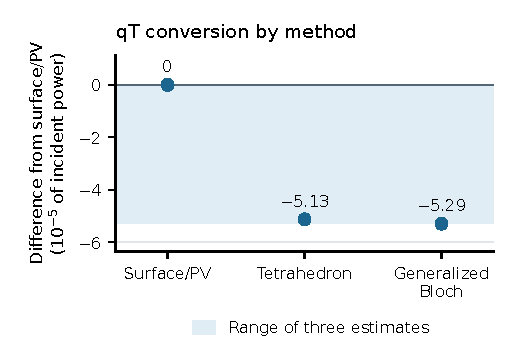
\includegraphics[width=0.53\linewidth]{figures/sm4_method_comparison.pdf}\par
 \small Companion to main-text Fig.~4. Each point gives the qT estimate minus the surface/PV estimate in units of $10^{-5}$ of incident power. Shading spans the three estimates.
\end{center}

Let $\widehat T_{\qT,j}$ denote the estimated qT conversion from method $j$. The three methods give
\begin{equation*}
 \min_j\widehat T_{\qT,j}\simeq0.12561,\qquad \max_j\widehat T_{\qT,j}\simeq0.12566.
 \tag{SM4a}\label{eq:s6-central-range}
\end{equation*}
The unrounded estimates differ by at most $0.0053$ percentage points of incident power. This spread measures agreement among methods. Establishing an error bound for the exact lattice solution requires separate evidence. All three methods give
\begin{equation*}
 T_{\qT}^{\rm modal}\simeq0.126.
 \tag{SM4b}\label{eq:s6-headline}
\end{equation*}
Using the four unrounded fractions from the reference calculation gives the power-balance residual
\begin{equation*}
 \left|R_q+T_q+T_{\qL}^{\rm modal}+T_{\qT}^{\rm modal}-1\right|
 \simeq1.30\times10^{-11}.
 \tag{SM4c}\label{eq:s6-closure}
\end{equation*}
The residual measures how closely the calculated outgoing powers sum to the incident power. A small residual alone cannot determine the accuracy of an individual channel or validate the Hamiltonian.

\paragraph*{Integration settings and separate convergence diagnostics.}

The controlling calculation combines an $N=192$ marching-surface co-area quadrature of the real-axis bulk level sets on a periodic reciprocal grid with an $M=256$ Jackson--Chebyshev principal-value reconstruction. The PV matrix is the equal mean of two independently scrambled Sobol samples, each with $2^{23}$ points (seeds 20260920 and 20260921), using 16384 energy bins on $[0,12]$ and Jackson margin 1.02. The samples use SciPy 1.17.0 \texttt{scipy.stats.qmc.Sobol} with scrambling enabled~\cite{SciPy2020}. The same samples supply the order ladder; larger same-seed samples extend nested prefixes rather than independent repetitions. At degenerate grid nodes, each tied branch receives its equal-rank share of the complete projected eigenspace weight before interpolation; geometric diagnostics retain the complete-cluster coherences. The validation records contain the raw matrices, basis-rotation controls and coverage diagnostics.

For sampler ensemble $r$, let $P_M^{(r)}$ be its principal-value matrix and $g_{00}^{(r)}(M)=[P_M^{(r)}]_{00}$, the $X_1$ source-sector diagonal entry. The tabulated definitions are
\begin{equation}
 \overline P_M=\frac12\sum_{r=1}^{2}P_M^{(r)},\qquad
 d_M=100\,\frac{\|\overline P_M-\overline P_{256}\|_F}{\|\overline P_{256}\|_F},\qquad
 s_{00}(M)=100\,\frac{\max_r g_{00}^{(r)}-\min_r g_{00}^{(r)}}{\frac12\sum_r g_{00}^{(r)}} .
\end{equation}
For the marching-surface matrix, $A_{\rm pre}$ denotes the raw complex assembly before reciprocal projection,
\begin{equation}
 A=\operatorname{Re}\!\left[\frac{A_{\rm pre}+A_{\rm pre}^{T}}2\right],\qquad
 \epsilon_{\rm sym}=\max\!\left[
 \frac{\|\operatorname{Im}A_{\rm pre}\|_F}{\max(\|\operatorname{Re}A_{\rm pre}\|_F,10^{-30})},
 \frac{\|A_{\rm pre}-A_{\rm pre}^{\dagger}\|_F}{\max(\|A_{\rm pre}\|_F,10^{-30})}
 \right].
\end{equation}
The listed minimum eigenvalue is evaluated after this projection. Here $\pi\rho_{\qT}^{\rm modal}=\ImH g_{0,0}^R+\ImH g_{0,1}^R$, $\pi\rho_{\qL}^{\rm modal}=\ImH g_{0,2}^R$, and $\rho_{\rm tot}=\rho_{\qT}^{\rm modal}+\rho_{\qL}^{\rm modal}$; $\epsilon_{\rm sym}$ separately measures the raw pre-projection residual. The wave-normal geometric-longitudinal matrix is retained only as a separately named diagnostic.

Table~\ref{tab:sm-physical-convergence} reports the physical six-segment ($12\times12$) kernel. The PV blocks and selected $N=192$ spectral block agree entry-for-entry with the corresponding leading blocks of the auxiliary ten-segment ($20\times20$) matrices; the spectral support-extension check was performed at this selected grid. Whole-matrix norms and eigenvalues are dimension specific.

\begin{table}[htbp]
\caption{Physical six-segment modal convergence diagnostics at $\omega=1.2$, with frequency conjugate to $\tau$. Percentages are shown for $d_M$ and $s_{00}$; the longitudinal norm is modal branch 2, not a wave-normal geometric projection.}
\label{tab:sm-physical-convergence}
\centering\scriptsize
\setlength{\tabcolsep}{2.6pt}
\renewcommand{\arraystretch}{0.98}
\begin{ruledtabular}
\begin{tabular}{rccc@{\hspace{7pt}}rcccc}
\multicolumn{4}{c}{principal-value order ladder}&\multicolumn{5}{c}{marching-surface ladder}\\
$M$&$\|\overline P_M\|_F$&$d_M$&$s_{00}$&$N$&$\|\pi\rho_{\rm tot}\|_F$&$\|\pi\rho_{\qL}^{\rm modal}\|_F$&$\lambda_{\min}(\rho_{\rm tot})$&$\epsilon_{\rm sym}$\\
\hline
192&0.896397&0.0513\%&0.0241\%&128&1.048264&0.113662&$4.12\times10^{-8}$&$2.13\times10^{-9}$\\
256&0.896608&0.0000\%&0.0601\%&160&1.048055&0.113676&$4.06\times10^{-8}$&$3.26\times10^{-9}$\\
320&0.896530&0.0155\%&0.1774\%&192&1.047933&0.113684&$4.03\times10^{-8}$&$5.40\times10^{-10}$\\
\end{tabular}
\end{ruledtabular}
\end{table}

The independent $N=192$ linear-tetrahedron calculation uses an unshifted periodic grid and the six-tetrahedron $000$--$111$ body-diagonal split. It linearly interpolates the sorted eigenvalues and uses centroid spectral weights with complete-projector rank sharing at ties. The analytic scalar retarded resolvent integral uses stable confluent divided differences with higher-precision fallbacks. Both signs of separation phase are retained when assembling the projected matrix. The choice $z=\omega^2+i10^{-10}$ selects the retarded logarithm branch rather than physical broadening. The surface and tetrahedron discretizations approximate the exact reciprocal-space integral.

The retained generalized-Bloch corroboration extrapolates the full complex projected Green matrix from finite $\eta$. In this numerical construction, the qL spectral block is taken from separately retained real-axis residues; the qT block is formed by subtracting that qL block from $\ImH g_0^R$ of the extrapolated matrix. This retained comparison can be replayed from the archived kernels; their original generator and its $\eta$ convention have not been identified from the retained records.


Table~\ref{tab:sm-high-resolution} compares the high-resolution qT sequences and generalized-Bloch extrapolations.

\begin{table}[htbp]
\caption{High-resolution modal-qT sequences and generalized-Bloch extrapolations. The spans are deterministic one-factor diagnostics and are not combined into a statistical error bar.}
\label{tab:sm-high-resolution}
\begin{ruledtabular}\begin{tabular}{lcc}
category & $T_{\qT}^{\rm modal}$ values & span\\\hline
surface/PV $N=128,160,192$ & $0.12567058,\ 0.12566614,\ 0.12565926$ & $1.133\times10^{-5}$\\
tetrahedron $N=128,160,192$ & $0.12559600,\ 0.12559347,\ 0.12560796$ & $1.450\times10^{-5}$\\
GB low-pair/quadratic/linear-LS & $0.12560631,\ 0.12559580,\ 0.12562207$ & $2.6276\times10^{-5}$\\
\end{tabular}\end{ruledtabular}
\end{table}
At fixed spectral grid $N=192$, changing the mean PV order from $M=192$ to $256$ changes qT by $0.00771\%$; increasing each Sobol sample from $2^{22}$ to $2^{23}$ points at $M=256$ changes it by $0.02355\%$. An independent two-shift $160^3$ PV sample mean differs from the selected result by $0.000158\%$. Higher orders increase the scramble and shift sensitivity. These are separate observed sensitivities, not a common statistical error bar.

The three central qT estimates span $0.12560631$--$0.12565926$. Surface refinement, PV sampling/order, tetrahedron refinement and retained generalized-Bloch extrapolation remain separate numerical categories. The controlling raw flux-closure residual is $1.30\times10^{-11}$. Neither the central spread nor flux closure is a complete numerical error bound; closure is an internal passivity and implementation check, not an independent validation of the Hamiltonian.


\paragraph*{Two profiles at fixed total stiffness.}
The fixed-total-stiffness comparison in main Sec.~6.1 uses the reference
profile and
$\bm g_{\rm end}/K_{\rm diag}=(0.5,0,0,0,0,0.5)$ at $\omega=1.2$.
All bare media and source positions are unchanged; $U$, $V$ and
$K_{\rm self}$ are rebuilt together from each complete paired-spring
profile before the reciprocal response is solved.  The calculation uses
the selected reference bare kernel: its $12\times12$ leading block is
in the order $(X_1,R_1,\ldots,X_6,R_6)$, with
$Q_{\qT}=\ImH g_{0,0}^R+\ImH g_{0,1}^R$ and
$Q_{\qL}=\ImH g_{0,2}^R$.  The geometrical transverse diagnostic is not
substituted for the modal qT power.

\begin{table}[htbp]
 \squeezetable
 \caption{Complete incident-power-normalized numerical partitions for
 the two profiles at fixed total spring stiffness.  The last column has
 total emitted bulk power as its denominator.  Central estimates are
 rounded for reproducibility; trailing digits are not certified precision.}
 \label{tab:sm-equal-total}
 \begin{ruledtabular}
 \begin{tabular}{lcccccc}
 Profile & $R_q$ & $T_q$ & $T_{\rm bulk}$
 & $T_{\qT}^{\rm modal}$ & $T_{\qL}^{\rm modal}$
 & $T_{\qT}^{\rm modal}/T_{\rm bulk}$\\
 \hline
 Reference & 0.0035721 & 0.8597460 & 0.1366819
 & 0.1256593 & 0.0110226 & 0.9193555\\
 Endpoint-only & 0.0550648 & 0.7618639 & 0.1830712
 & 0.1585773 & 0.0244939 & 0.8662055\\
 \end{tabular}
 \end{ruledtabular}
\end{table}

The reference partition reproduces the archived selected-kernel result
within $2.8\times10^{-17}$ absolutely; the largest four-channel closure
residual for these two states is $1.36\times10^{-11}$.  These are
regression and internal-consistency checks, not error bounds for the
lattice integration.  The separate revision-validation record for this comparison binds the
selected $N=192$ spectral and $M=256$ PV inputs, source conventions and
two separately solved coupled responses.  No additional kernel integration
or endpoint packet evolution was performed.  The endpoint-only profile
is outside the reference $\pm5\%$ coupling box, and its numerical
partition is not an inherited robustness certificate or an
endpoint-specific exact-lattice enclosure.  This pair is separate from
the original five-profile/85-case screen in SM5A. The two-profile comparison was added after the reference tolerance calculation. Its inputs and results are recorded under \nolinkurl{validation/significance/tradeoff_validation/} in the accompanying repository.

Returning to the reference profile, define the separately dressed surrogate family by $H_c(\alpha)=H_X+\alpha H_R$, with complete Hamiltonian $H(\alpha)=H_q+H_b+H_c(\alpha)$. Thus $\alpha$ multiplies the complete positive radial part of the coupling sector, including its core stiffness, line--core coupling, and line self-stiffness, while $H_q$ and $H_b$ remain fixed. Each point is therefore a new dressed complete solve. The 21-point sampled qT trend is shown in Fig.~\ref{fig:sm-alpha}; it is not an analytic monotonicity theorem.

\begin{figure}[htbp]
\centering
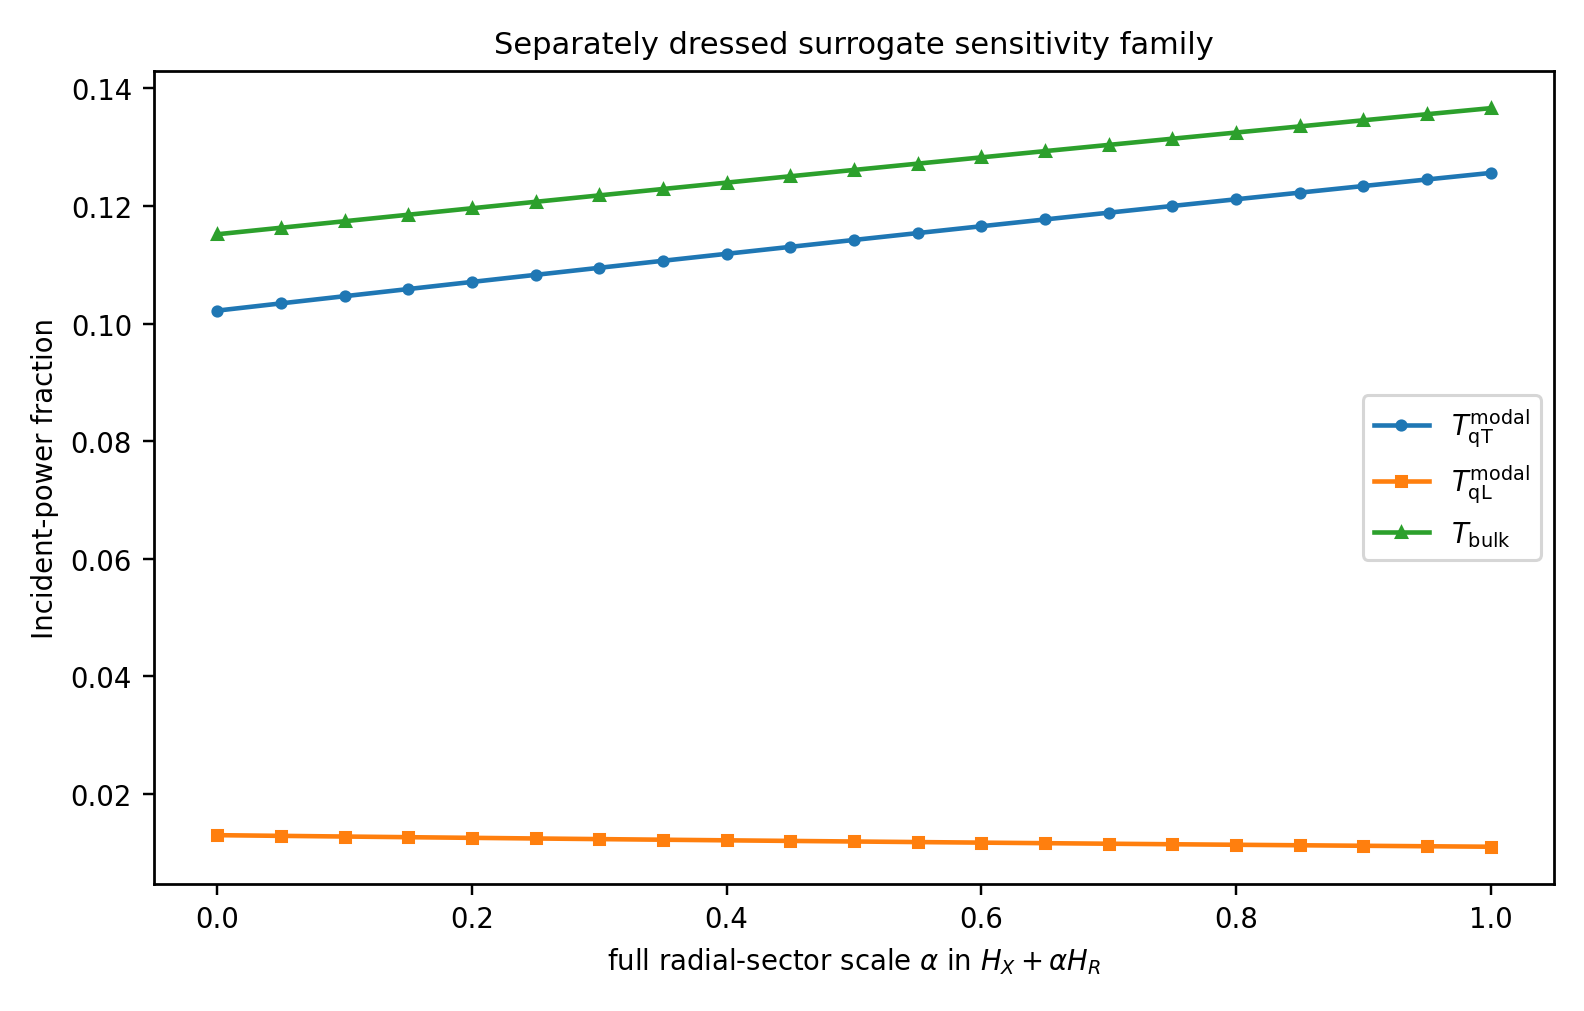
\includegraphics[width=0.72\linewidth]{figures/Halpha_transmission_scan_p06.png}
\caption{Separately dressed $H(\alpha)$ surrogate family at the reference frequency conjugate to $\tau$.}
\label{fig:sm-alpha}
\end{figure}

For the physical full state, decompose $V=V_X+V_R$ and set $\veta_\nu=(I+Ug_0^R)^{-1}V_\nu\vchi_D^{(L)}$ for $\nu\in\{X,R\}$, so that $\veta=\veta_X+\veta_R$. With $Q_{\qT}=\ImH g_{0,\qT}^R$, define $T_{\nu\nu}=2\veta_\nu^\dagger Q_{\qT}\veta_\nu$ and $T_{XR}=4\operatorname{Re}(\veta_X^\dagger Q_{\qT}\veta_R)$. The common-dressing decomposition obeys
\begin{equation}
 T_{\qT}^{\rm modal}=T_{XX}+T_{RR}+T_{XR}.
\end{equation}
At the controlling surface/PV point,
\begin{equation}
 (T_{XX},T_{RR},T_{XR})
 \simeq(0.10147813,0.00179177,0.02238935).
\end{equation}
The independent $N=192$ tetrahedron cross term differs by $0.026\%$. These are terms in one quadratic form, not separately conserved energies or the separately dressed ablation rows.

\paragraph*{Prescribed-source continuum comparison.}
The undressed continuum benchmark uses the pure-Bloch transforms $\widetilde{\vf}^{\rm slab}_X(\vk;\kappa)$ and $\widetilde{\vf}^{\rm slab}_R(\vk;\kappa)$ from SM1, with their displayed relative sign and phase retained. In local line coordinates take $Q_j=Qe^{i\kappa ja}$ for $j=0,\ldots,6$, segment midpoints $(s-\tfrac12)a$ for $s=1,\ldots,6$, and $(g_1,\ldots,g_6)=(0.1,0.2,0.2,0.2,0.2,0.1)$. The numerical reference units are $a=Q=1$, $\omega=1.2$, $\kappa a=0.9594572753515053$, $c_T=1$, and $c_L=\sqrt3$. Write $\widetilde{\vf}_\nu=\widetilde{\vf}^{\rm slab}_\nu(\vk;\kappa)$ and $\widetilde{\vf}=\widetilde{\vf}_X+\widetilde{\vf}_R$. Equivalently, this is the Fourier transform of the bare physical corner force $-BV\bm Q_D$, where $\bm Q_D=(Q_0,\ldots,Q_6)^T$ and $B,V$ are the main text's centered basis and mixed stiffness block. It includes neither core feedback nor the dressed line response.

For a unit direction $\bm n$, define the relative compressional and shear power functionals
\begin{align}
 W_P[\widetilde{\vf}]&=c_L^{-3}\int_{S^2}
 \left|\bm n\cdot\widetilde{\vf}\bigl((\omega/c_L)\bm n\bigr)\right|^2\,d\Omega,\nonumber\\
 W_S[\widetilde{\vf}]&=c_T^{-3}\int_{S^2}
 \left[\left\|\widetilde{\vf}\bigl((\omega/c_T)\bm n\bigr)\right\|^2
 -\left|\bm n\cdot\widetilde{\vf}\bigl((\omega/c_T)\bm n\bigr)\right|^2\right]d\Omega,\nonumber\\
 s_S[\widetilde{\vf}]&=\frac{W_S[\widetilde{\vf}]}{W_P[\widetilde{\vf}]+W_S[\widetilde{\vf}]}.
 \label{eq:sm-continuum-weights}
\end{align}
The two source evaluations lie on different wave-number spheres. With continuum density $\rho_m=m_b/a^3$ and the phasor convention of SM3, physical radiation power is $P_C=\omega^2W_C/(32\pi^2\rho_m)$ for $C=P,S$. This follows by applying the work identity to the isotropic continuum spectral measure: radial integration of $\delta(c_C^2k^2-\omega^2)$ gives $\omega/(2c_C^3)$, with $c_P=c_L$ and $c_S=c_T$. The common prefactor cancels from $s_S$; these prescribed-force weights are not incident-line-normalized transmission coefficients.

Define $W_{C,\nu\nu}=W_C[\widetilde{\vf}_\nu]$ and $W_{C,XR}=W_C[\widetilde{\vf}_X+\widetilde{\vf}_R]-W_{C,XX}-W_{C,RR}$. Table~\ref{tab:sm-continuum-interference} resolves the coherent comparison. The X-only shear share is $0.87495206$ and the R-only share is $0.91771932$. Summing only the two self terms gives $0.87636169$, whereas their coherent sum gives $0.91914369$: the interference is constructive for S and destructive for P. Its S cross term is $24.48\%$ of coherent continuum S power, distinct from the $17.8\%$ same-state dressed lattice qT cross term above. The agreement of the final continuum and lattice shares does not equate their dispersion, dressing, or absolute transmission.

\begin{table}[htbp]
\caption{Relative continuum radiation weights for the prescribed $Q=1$ source. The common physical-power prefactor is omitted; cross terms are contributions to one coherent quadratic form.}
\label{tab:sm-continuum-interference}
\begin{ruledtabular}
\begin{tabular}{lrr}
source term & $W_S$ & $W_P$\\\hline
$XX$ & $9.81946085$ & $1.40339500$\\
$RR$ & $0.35104365$ & $0.03147380$\\
$XR$ & $3.29640150$ & $-0.25019629$\\
\end{tabular}
\end{ruledtabular}
\end{table}

The archived continuum producer uses Gauss--Legendre quadrature in $\mu=n_x$ and midpoint sampling in azimuth, with $(n_\mu,n_\phi)=(60,120),(120,360),(240,720)$. An independent evaluation of the self and cross terms on $(40,80),(80,160),(160,320)$ reproduces the displayed shares, with a share spread below $3\times10^{-15}$. This is observed quadrature agreement, not a rigorous error enclosure.

For comparison, evaluating the main text's weak-coupling spectral ratio with the selected six-segment surface kernel gives $\mathcal A_{\qT}=0.0969632610$, $\mathcal A_{\qL}=0.0076249508$, and limiting share $0.92709550$; the independent $N=192$ tetrahedron kernel gives $0.92712205$. The coefficients use $\veta_{c,1}=V_1G_{D,0}^R\sqrt{\gamma_q}|L\rangle$ with Caroli normalization. A selected-kernel solve at $s=0.001$ gives share $0.92708565$, consistent with this fixed-frequency limit. These are numerical evaluations using retained spectral matrices, not new certified bounds. Weak coupling retains the lattice spectral measure; replacing it by isotropic continuum shells is a separate approximation and does not establish a continuum limit for the finite-coupling junction.

Figure~\ref{fig:sm-continuum} compares the continuum shear fractions with the lattice generated-bulk qT share.

\begin{figure}[htbp]
\centering
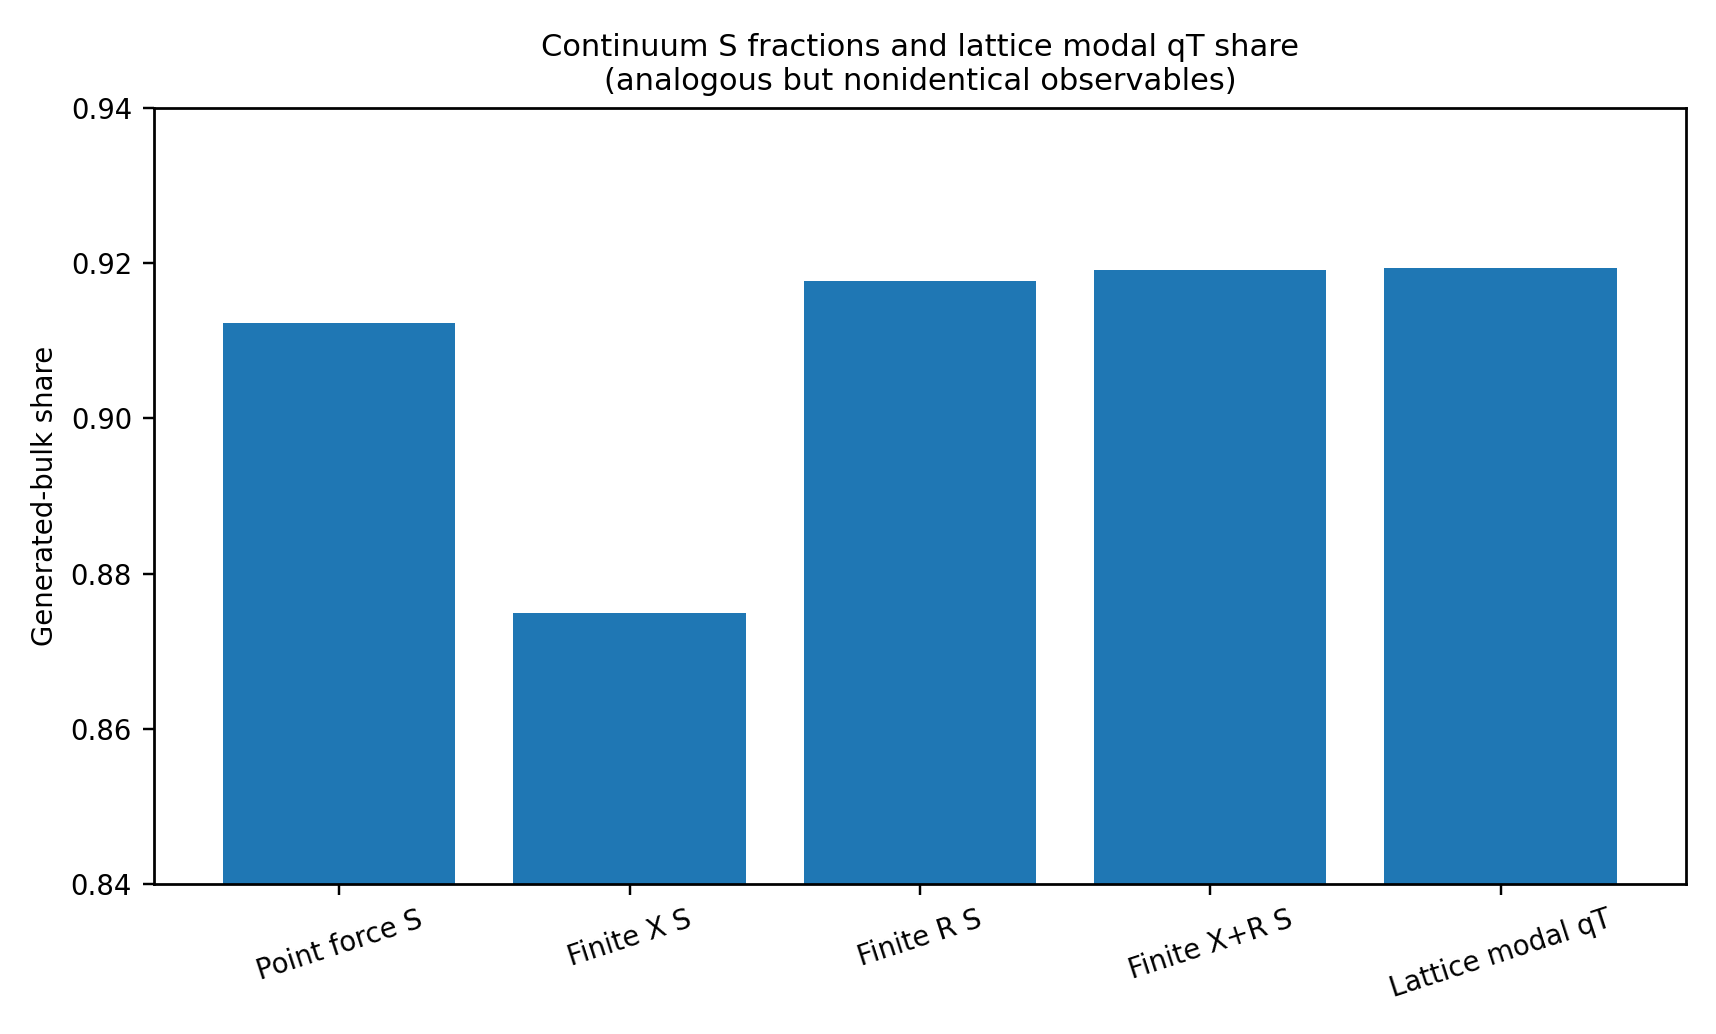
\includegraphics[width=0.72\linewidth]{figures/continuum_lattice_share_comparison_p06.png}
\caption{Continuum shear fractions and the lattice modal-qT generated-bulk share. These are analogous but nonidentical observables and the comparison does not derive the absolute lattice transmission.}
\label{fig:sm-continuum}
\end{figure}

\section{Branch-resolved modal robustness and scalar real-time controls}

\subsection{Finite parameter families}

The branch-resolved robustness calculations use
\begin{equation}
 \ImH g_{0,\qT}^R=\ImH g_{0,0}^R+\ImH g_{0,1}^R,
 \qquad
 \ImH g_{0,\qL}^R=\ImH g_{0,2}^R.
\end{equation}
Table~\ref{tab:sm-modal-robust} gives the exact finite one-factor inputs; positivity on these grids is not a theorem over a continuous interval.

\begin{table}[!htbp]
\caption{Exact branch-resolved modal-qT robustness inputs; ranges refer only to the finite tested values. Frequencies and line speeds use Hamiltonian time $\tau$, with the equilibrium spacing $a$ as the length unit.}
\label{tab:sm-modal-robust}
\centering\scriptsize\setlength{\tabcolsep}{2.8pt}\renewcommand{\arraystretch}{0.96}
\begin{tabular}{@{}llccc@{}}\toprule
family&exact tested values&count&method&qT range\\\midrule
frequency&$\omega=0.600+0.025j$, $j=0,\ldots,48$&49&M2&0.10486--0.21774\\
coupling&$s=(0.05,0.075,0.10,0.15,0.20,0.25,0.50,1.00,1.50,2.00)$&10&M1&0.000246--0.52218\\
slab length&$N_c=(2,3,4,6,8,10)$; rule below&6&M1&0.00882--0.24512\\
profile&five six-segment vectors below&5&M1&0.06495--0.15787\\
line speed&$c_q=(0.65,0.8,0.9,1.0,1.1,1.2,1.3,1.5,1.7,2.0)$&10&M1&0.02646--0.12569\\
stiffness&$K_{\rm diag}/K_{\rm axis}=(0.75,0.9,1.0,1.1,1.25)$&5&M3&0.09815--0.16902\\\bottomrule
\end{tabular}

\parbox{0.99\linewidth}{\scriptsize Except where varied, $a=m_q=m_b=K_{\rm axis}=K_{\rm diag}=1$, $K_q=1.69$ ($c_q=1.3$), $\omega=1.2$, $N_c=6$, and $\bm g_{\rm ref}=(0.10,0.20,0.20,0.20,0.20,0.10)$ are fixed. M1, M2, and M3 use (PV order, surface grid) $(256,80)$, $(256,80)$, and $(160,80)$. The common medium uses the two $2^{23}$-point Sobol samples above. Each stiffness case uses its own two shifted $64^3$ grids and $2^{19}$-point Sobol sample with 6144 bins on the full spectral support $[0,(4K_{\rm axis}+8K_{\rm diag})/m_b]$; exact shifts and seeds are recorded in the archive. For $N_c=2$, $\bm g=(0.10,0.10)$; otherwise endpoints are 0.10 and interiors 0.20. Other profiles are $\bm g_{\rm uniform}=(0.20,0.20,0.20,0.20,0.20,0.20)$, $\bm g_{\rm soft}=(0.05,0.12,0.20,0.20,0.12,0.05)$, $\bm g_{\rm short}=(0,0.10,0.20,0.20,0.10,0)$, and $\bm g_{\rm edge}=(0.20,0.10,0.10,0.10,0.10,0.20)$. In the coupling family $s$ scales the reference profile and $s=0$ is a separate exact null. In the speed family $a=m_q=1$ and $K_q=c_q^2$. The stiffness family varies $K_{\rm diag}$ at fixed $K_{\rm axis}=1$, retaining the reference time and energy units and the stated values of $K_q$, $\omega$, and $\bm g_{\rm ref}$. Complete row-level values, numerical encodings, and producer inputs are provided in the validation archive.}
\end{table}

All 85 sampled positive-coupling qT values are positive; qL is nonnegative; the largest flux-closure residual is $3.97\times10^{-11}$; and the largest $T_{\qT}+T_{\qL}-T_{\rm bulk}$ residual is $8.33\times10^{-17}$. The exact zero-coupling control gives zero bulk output. The sampled weak-coupling log slope is $2.0315$; the analytic modal theorem, rather than this coarse slope, controls the sufficiently-small-coupling existence statement. The finite-reference neighborhood statement follows separately from continuity of the fixed-topology response and the verified regularity margins. The five spacing values listed in main Sec.~8.1 are dimensional re-encodings of one unchanged nondimensional calculation and are not included among the 85 positive-coupling cases. Their exact equality is a units-covariance check, not a physical parameter sweep, refinement, or continuum convergence. Complete current row values and method records, together with the retained analytic shell and branch checks, are provided in the validation archive.

\subsection{A bound for simultaneous segment-coupling changes}
\label{sec:sm-coupling-box}

Fix the reference frequency, bare media and geometry, and put $g_s=g_s^\star(1+\delta_s)$, $|\delta_s|\leq e_s<1$. The eight equal links within each segment vary together. The archive already contains random six-coupling profile tests; the following bound controls the complete box for fixed Green matrices.

Use the 12-coordinate centered source basis and the seven line coordinates. Write $g_0=g_0^R(\omega)$, $Q=\ImH g_{0,\qT}^R\succeq0$, and $h=\omega^2M_D-K_D-K_{\rm self}-\Sigma_L^R-\Sigma_R^R$. With a fixed reference stiffness $k_\star>0$, the dimensionless response satisfies
\begin{equation}
 y=\binom{\sqrt{k_\star}\vchi_D^{(L)}}{\veta_c/\sqrt{k_\star}},\qquad
 \mathcal A(\bm\delta)y=b,\qquad
 \mathcal A=
 \begin{pmatrix}h/k_\star&V^\dagger g_0\\-V/k_\star&I+Ug_0\end{pmatrix},\qquad
 b=\binom{\sqrt{\gamma_q/k_\star}|L\rangle}{0}.
 \label{eq:sm-box-system}
\end{equation}
The segment Hessians make $\mathcal A=\mathcal A_0+\sum_s\delta_s\mathcal A_s$ affine in the coupling errors. Assume $\mathcal A_0$ is invertible. Let $y_0=\mathcal A_0^{-1}b$, $\mathcal B(\bm\delta)=\mathcal A_0^{-1}(\mathcal A-\mathcal A_0)$, and $F=\sqrt{2k_\star}\,Q^{1/2}P_\eta$, where $P_\eta$ extracts the lower twelve coordinates. Thus $T_{\qT}^{\rm modal}=\|Fy\|_2^2$.

Let $\mathcal V$ contain the 64 box vertices, $\delta_s=\pm e_s$, and put $\mathcal W_0=I+U_0g_0$. The intermediate core inverse used in the eliminated response exists throughout the box if $\mathcal W_0$ is invertible and
\begin{equation}
 r_c=\max_{\mathcal V}\|\mathcal W_0^{-1}(U-U_0)g_0\|_2<1.
 \label{eq:sm-box-core}
\end{equation}
Define
\begin{align}
 r&=\max_{\mathcal V}\|\mathcal B\|_2,&
 v&=\max_{\mathcal V}\|\mathcal B y_0\|_2,\\
 w&=\max_{\mathcal V}\|F\mathcal B\|_2,&
 d_{\rm out}&=\max_{\mathcal V}\|F\mathcal B y_0\|_2.
 \label{eq:sm-box-maxima}
\end{align}
Each norm is convex in $\bm\delta$, so its largest vertex value bounds it throughout the box. If $r<1$, the exact identity
\begin{equation}
 y=y_0-\mathcal B y_0+\mathcal B(I+\mathcal B)^{-1}\mathcal B y_0
\end{equation}
and $\|(I+\mathcal B)^{-1}\|_2\leq(1-r)^{-1}$ imply
\begin{equation}
 \|F(y-y_0)\|_2\leq d_{\rm out}+\frac{wv}{1-r},\qquad
 T_{\qT}^{\rm modal}(\bm\delta)\geq
 \left[\max\left(0,\|Fy_0\|_2-d_{\rm out}-\frac{wv}{1-r}\right)\right]^2.
 \label{eq:sm-box-floor}
\end{equation}
This retains the leading change in the output norm instead of bounding it through the full state norm. The convexity argument concerns the four auxiliary norms; it does not require transmission extrema to occur at vertices.

For $e_s=0.05$ and $k_\star=K_q=1.69$, the reference $N=192$, $M=256$ matrices give $r_c\simeq0.00573$, $r\simeq0.0563$, and an output-amplitude error bound of $0.02579$, yielding the numerical floor in Table~\ref{tab:sm-box-floor}. An outward-rounded evaluation on the exact dyadic representations of the supplied matrices gives a lower floor greater than $0.10804017$, certifying $T_{\qT}^{\rm modal}>27/250=0.108$ throughout the same coupling box.

\begin{table}[htbp]
\centering
\caption{Numerically evaluated conditional bounds for simultaneous $\pm5\%$ changes in all six segment couplings at $\omega=1.2$, with frequency conjugate to $\tau$. Each row uses its fixed computed bulk matrices.}
\label{tab:sm-box-floor}
\begin{tabular}{lcc}
\toprule
Bulk calculation & Reference $T_{\qT}^{\rm modal}$ & Whole-box floor\\
\midrule
Surface $N=128$, PV $M=256$ & $0.125671$ & $0.108048$\\
Surface $N=192$, PV $M=256$ & $0.125659$ & $0.108040$\\
Tetrahedron $N=192$ & $0.125608$ & $0.107999$\\
\bottomrule
\end{tabular}
\end{table}

The 18 configurations varying surface grid, PV order, sample size and sampling rule, and tetrahedron resolution give numerical floors $0.1079863$--$0.1080508$. These shared-input evaluations measure sensitivity. To transfer the selected finite-matrix certificate to the infinite lattice, let a subscript $c$ denote its cached matrices and response, and define
\begin{equation}
 \Delta G=k_\star(g_0-g_{0,c}),\quad
 \Delta Q_\star=k_\star(Q-Q_c),\quad
 e_G=\|\Delta G\|_2\leq\frac1{50},\quad
 e_Q=\|\Delta Q_\star\|_2\leq\frac1{200}.
 \label{eq:sm-certified-kernel-errors}
\end{equation}
Validated contour integration certifies these inequalities at $\omega=1.2$ over all three angular charts, including the regular exterior contribution to $g_0$. The comparison uses every entry of the actual cached matrices. The exact $Q\succeq0$ follows from its positive lower-cluster spectral measure, including complete tied eigenspaces. The contour identities, outward integral enclosures and executable checks are provided in the validation archive.

Here the quantities in Eqs.~\eqref{eq:sm-box-core}--\eqref{eq:sm-box-maxima} refer to the cached response. Put $\mathcal R_c=\mathcal A_{0,c}^{-1}$ and $D_g=k_\star^{-1}\binom{V^\dagger}{U}$. Then $\mathcal A=\mathcal A_c+D_g\Delta G P_\eta$. Define the additional vertex bounds
\begin{align}
 h_g&=\max_{\mathcal V}\|\mathcal R_cD_g\|_2,&
 h_c&=\max_{\mathcal V}\|\mathcal W_{0,c}^{-1}U/k_\star\|_2,\\
 d_\eta&=\max_{\mathcal V}\|P_\eta\mathcal B y_{0,c}\|_2,&
 w_\eta&=\max_{\mathcal V}\|P_\eta\mathcal B\|_2.
\end{align}
Convexity extends these bounds throughout the coupling box. With
\begin{align}
 L&=\|F_cy_{0,c}\|_2-d_{\rm out}-\frac{wv}{1-r},&
 Z&=\|P_\eta y_{0,c}\|_2+d_\eta+\frac{w_\eta v}{1-r},\\
 \rho&=r+h_ge_G,&
 \sigma&=\frac{h_ge_G Z}{1-\rho},
\end{align}
the same inverse identity gives $\|y-y_c\|_2\leq\sigma$ when $\rho<1$. The core inverse also persists if $r_c+h_ce_G<1$. Hence, when $L>\|F_c\|_2\sigma$,
\begin{equation}
 T_{\qT}^{\rm modal}\geq
 (L-\|F_c\|_2\sigma)^2-2e_Q(Z+\sigma)^2
 >\frac{1037}{10000}.
 \label{eq:sm-certified-lattice-floor}
\end{equation}
The first term bounds the squared cached output norm of the perturbed state; the second bounds the change of spectral matrix. An outward-rounded replay verifies both inverse conditions and the last inequality using Eq.~\eqref{eq:sm-certified-kernel-errors}. This certifies the infinite-lattice reference-frequency floor throughout the same six-coupling box.

\subsection{Packet preparation, estimator, and numerical controls}
\label{sec:sm-packet-controls}

The reference packet evolves in the six-segment taper. Section~SM5D gives the independent run for the increasing ramp. Both start from the same real, right-moving line preparation.

\paragraph*{Preparation and incident energy.}
At $\tau=0$, set
\begin{equation*}
 \begin{aligned}
 q_i(0)&=A e^{-(ia-x_c)^2/(2\sigma_x^2)}\cos[\kappa_0(ia-x_c)],\\
 (A,x_c,\sigma_x)&=(0.002a,18a,7a).
 \end{aligned}
 \tag{SM5Ca}\label{eq:s7-packet}
\end{equation*}
The uncoupled line dispersion gives $\kappa_0a\simeq0.9594572754$ at $\omega_0=1.2$. Here $E_0=H_q(0)$ is the prepared open-line energy and $E_{\rm link}(\tau)=H_c(\tau)$ is the complete source-link energy. Initially $E_{\rm link}(0)/E_0=2.05\times10^{-18}$ for the reference taper.

For the initial real packet, let $N_{\rm line}$ be the number of line sites in the periodic Parseval representation and use the discrete Fourier transform (DFT) pair
\begin{equation}
 \widehat q(k)=\sum_{j=0}^{N_{\rm line}-1}q_j e^{-ikja},
 \qquad
 q_j=\frac{1}{N_{\rm line}}\sum_k\widehat q(k)e^{ikja},
 \label{eq:s7-line-dft}
\end{equation}
with the same convention for $\widehat{\dot q}$. For $0<|k|a<\pi$ the sign of the group velocity $v_{g,q}(k)=\partial\omega_q(k)/\partial k$ selects the traveling component,
\begin{equation*}
 \widehat{\dot q}(k,0)=-i\,\operatorname{sgn}[v_{g,q}(k)]\,\omega_q(k)\widehat q(k,0).
 \tag{SM5Cb}\label{eq:s7-packet-velocity}
\end{equation*}
The velocity coefficients at zero and Nyquist wavenumber are set to zero. Every bulk site starts at its equilibrium position with zero velocity,
\begin{equation*}
 \bm u_{\bm r}(0)=\dot{\bm u}_{\bm r}(0)=0.
 \tag{SM5Cc}\label{eq:s7-unexcited-bulk}
\end{equation*}
The full-grid spectral-energy weights are
\begin{equation}
 W(k)=\frac{m_q}{2N_{\rm line}}\left(|\widehat{\dot q}(k,0)|^2+\omega_q^2(k)|\widehat q(k,0)|^2\right).
 \label{eq:sm-packet-weight}
\end{equation}
The $\pm k$ coefficients are the conjugate representation of one real right-moving packet, not two launched inputs. The packet transmission formula in main-text Sec.~7 uses both signed members of every propagating pair in its numerator and the full periodic Parseval energy in its denominator. The frequencies at the $1\%$ and $99\%$ energy quantiles are approximately $0.932$ and $1.473$. The zero-frequency component has zero energy for this preparation. The stationary Nyquist component is excluded from the numerator but retains its stored energy in the denominator. The reported right-moving fraction is $0.9999997423$; the remaining $2.58\times10^{-7}$ is the stationary Nyquist energy fraction. The periodic Parseval energy differs from the open-line $H_q(0)$ by $9.18\times10^{-9}$ relatively because the periodic representation contains a closing bond absent from the open production line.

\paragraph*{Choice of time interval.}
The finite dynamics advances both subsystems with the symmetric velocity-Verlet scheme and no external drive or damping after preparation. For the interval selection, $J_{q\to b}$ sums the signed currents of the physical source links, each counted once from the line toward the bulk. The velocity at a line endpoint is $\dot q_i\hat{\bm x}$. The energy of the open bulk is $E_b^{\rm open}=H_b$ with its free-face bond inventory. The corresponding periodic diagnostic energy $E_{\rm bulk}^{\rm per}$ is computed on the same snapshot by Eq.~\eqref{eq:s7-periodic-total-energy}. The two-cell transverse ($y,z$) boundary strips contain the fraction $f_{\rm shell}^{\rm kin}$ of total bulk kinetic energy. A sampled time qualifies when it satisfies all five conditions
\begin{equation*}
 \begin{aligned}
 E_{\rm link}/E_0&\le2.5\times10^{-3},&
 |J_{q\to b}|/E_0&\le5.0\times10^{-4},\\
 f_{\rm shell}^{\rm kin}&\le2.0\times10^{-3},&
 \delta_{\rm per/open}&\le2.5\times10^{-3},\\
 |H(\tau)-H(0)|/H(0)&\le10^{-5}.
 \end{aligned}
 \tag{SM5Cd}\label{eq:s7-selector-a}
\end{equation*}
Here
\begin{equation*}
 \delta_{\rm per/open}=\frac{|E_{\rm bulk}^{\rm per}-E_b^{\rm open}|}{E_b^{\rm open}}.
 \tag{SM5Ce}\label{eq:s7-selector-b}
\end{equation*}
The threshold on $|J_{q\to b}|/E_0$ is in inverse units of $\tau$. The remaining four conditions are dimensionless. The reference search examines $48\le\tau\le57$ at cadence $0.2$, accepts runs of duration at least $2.0$, and selects the longest passing run with the earliest start in a tie. The five conditions use only the direct simulation. They give the interval
\begin{equation*}
 52.8\le\tau\le55.4.
 \tag{SM5Cf}\label{eq:s7-window}
\end{equation*}
Section~\ref{sec:sm-perspectives} explains how to retain the selected events when changing the time coordinate. A separate post-selection check includes the union of all six face shells, assigning each node its kinetic energy and half the energy of each incident bulk bond. The production and larger-box shell maxima over Eq.~\eqref{eq:s7-window} are reported below.

Figure~\ref{fig:sm-packet-selection} shows how the five criteria select the reference taper's interval independently of the stationary prediction. The stored qT fraction is averaged over the selected snapshots by the composite trapezoidal rule specified below.

\begin{figure}[htbp]
 \centering
 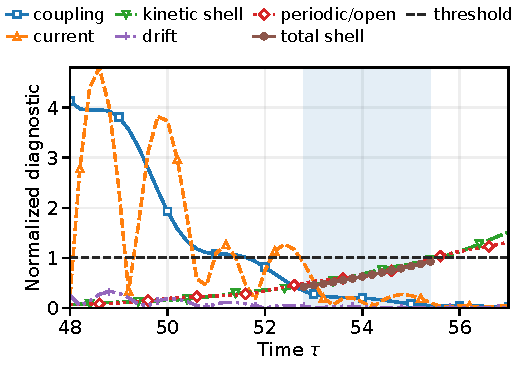
\includegraphics[width=0.57\linewidth]{figures/paper1_sectionVII_fig6b_selector_controls_v2.pdf}
 \caption{Selection of the reference packet interval in time $\tau$, in units of $\sqrt{m_b/K_{\rm diag}}$. The five diagnostics in Eq.~\eqref{eq:s7-selector-a} are each divided by their own threshold. All five must be at or below the dashed line at one. The total-shell points show the separate six-face check performed after selection. Main-text Fig.~6 shows the stored qT energy over the same interval.}
 \label{fig:sm-packet-selection}
\end{figure}

\paragraph*{Modal allocation at each snapshot.}
For the periodic bulk diagnostic, let $N=N_xN_yN_z$, let $\bm n$ denote its integer cell indices, and use
\begin{equation}
 \widehat{\bm u}(\vk)=\sum_{\bm n}\bm u_{\bm n}e^{-i\vk\cdot a\bm n},
 \qquad
 \bm u_{\bm n}=\frac{1}{N}\sum_{\vk}\widehat{\bm u}(\vk)e^{i\vk\cdot a\bm n},
 \label{eq:s7-bulk-dft}
\end{equation}
with the same convention for $\widehat{\dot{\bm u}}$. With $D(\vk)$ the mass-normalized bulk dynamical matrix, the energy of this periodic embedding is
\begin{equation}
 E_{\rm bulk}^{\rm per}
 =\frac{m_b}{2N}\sum_{\vk}
 \left[
  \widehat{\dot{\bm u}}^{\dagger}\widehat{\dot{\bm u}}
  +\widehat{\bm u}^{\dagger}D(\vk)\widehat{\bm u}
 \right].
 \label{eq:s7-periodic-total-energy}
\end{equation}
For an isolated upper branch the qL energy at a wavevector follows by projecting onto its unit polarization $\bm e_2$. In the absence of upper--middle ties the corresponding whole-grid formulas are
\begin{equation*}
 \begin{aligned}
 E_{\qL}^{\rm per}
 &=\frac{m_b}{2N}\sum_{\bm k}
 \left[|\bm e_2^\dagger\widehat{\dot{\bm u}}|^2+\omega_2^2|\bm e_2^\dagger\widehat{\bm u}|^2\right],\\
 E_{\qT}^{\rm per}&=E_{\rm bulk}^{\rm per}-E_{\qL}^{\rm per}.
 \end{aligned}
 \tag{SM5Cg}\label{eq:s7-modal-energy}
\end{equation*}
At an exact degenerate eigenspace $d$, let $\mathsf E_d$ contain orthonormal polarization columns, let $\lambda_d=\omega_d^2$ be the common squared frequency, and define $\bm c_u=\mathsf E_d^\dagger\widehat{\bm u}$ and $\bm c_v=\mathsf E_d^\dagger\widehat{\dot{\bm u}}$. The energy-coherence matrix is
\begin{equation}
 \mathcal C_d=\frac{m_b}{2N}
 \left(\bm c_v\bm c_v^\dagger+\lambda_d\bm c_u\bm c_u^\dagger\right).
\end{equation}
For any normalized one-dimensional direction $\bm z$ inside that eigenspace, the allocated energy $\bm z^\dagger\mathcal C_d\bm z$ lies between the minimum and maximum eigenvalues of $\mathcal C_d$. The numerical classifier uses a relative squared-frequency tolerance $10^{-12}$ and retains the full classified block rather than selecting an arbitrary branch basis.

Let $\mathcal E_{\qT}^{\rm TD}(\tau)=E_{\qT}^{\rm per}(\tau)/E_0$. For the stored cadence $h=0.2$, set $N_h=(\tau_b-\tau_a)/h$ and $\mathcal E_j=\mathcal E_{\qT}^{\rm TD}(\tau_a+jh)$ for $j=0,\ldots,N_h$. The reported average is the composite-trapezoidal value $\overline{\mathcal E}_{\qT,h}^{\rm TD}=h[(\mathcal E_0+\mathcal E_{N_h})/2+\sum_{j=1}^{N_h-1}\mathcal E_j]/(\tau_b-\tau_a)$. Invariant treatment of 132 upper--middle doublets and 231 threefold points gives
\begin{equation}
 0.12762638643388616\le\overline{\mathcal E}_{\qT,h}^{\rm TD}
 \le0.12762638738500592.
 \label{eq:s7-direct-result}
\end{equation}
The decimal midpoint of these cadence-$0.2$ allocation bounds is $0.12762638690944604$; it is not an exact continuous-time average. It is reported as approximately $0.1276263869$ in numerical prose and $0.1276$ in physical interpretation. The interval width is below $9.52\times10^{-10}$ of $E_0$ and concerns only allocation within degenerate subspaces. The sampled instantaneous range is $0.1274833$--$0.1277449$. The corresponding cadence-$0.2$ qL and periodic-bulk trapezoidal averages are $0.0113021$ and $0.1389284$.

\paragraph*{Stationary packet comparison.}
Let $\mathcal G$ be the full signed line-DFT grid and $\mathcal P=\{k\in\mathcal G:0<|k|a<\pi\}$. All fourteen distinct DFT frequencies in $\mathcal K=\{k\in\mathcal P:0.8\le\omega_q(k)\le1.6\}$ are evaluated directly, with packet-energy coverage $c_{\mathcal K}=\sum_{k\in\mathcal K}W(k)/\sum_{k\in\mathcal G}W(k)=0.9996834928$. Adding the represented propagating bins at their own frequencies uses the full initial periodic energy as the denominator,
\[
 S_{C,\mathcal K}=
 \frac{\sum_{k\in\mathcal K}W(k)T_C[\omega_q(k)]}{\sum_{k\in\mathcal G}W(k)}.
\]
These in-band contributions require no frequency interpolation. Figure~6 in the main text overlays the surface result at $N=160$ with principal-value reconstruction order $M=256$, and the range between that result and the $N=128$ tetrahedron result. The values of $S_{\qT,\mathcal K}$ are $0.1276811,0.1276730$ for surface grids $N=128,160$ and $0.1275676,0.1275947,0.1276094$ for tetrahedron grids $N=96,128,160$. The difference between the direct average and the selected surface contribution is about $0.0365\%$ relative to that surface prediction. Energy-weighted absolute nodewise differences, divided by the finer-grid contribution, are $0.00636\%$ for surface refinement and $0.02581\%,0.01218\%$ for successive tetrahedron refinements. Relative to the selected surface contribution, the tetrahedron $N=128$ and $160$ results differ by $0.06137\%$ and $0.04981\%$, respectively. These observed differences do not bound the exact integration error. Passivity bounds each omitted propagating coefficient by $0\le T_C\le1$. The combined weight of the omitted propagating bins is at most $1-c_{\mathcal K}$, which also includes the stationary Nyquist weight. It follows that
\begin{equation*}
 S_{C,\mathcal K}\le T_C^{\rm packet}\le S_{C,\mathcal K}+1-c_{\mathcal K}.
 \tag{SM5Ch}\label{eq:s7-packet-tail-bound}
\end{equation*}
For the selected surface result, Eq.~\eqref{eq:s7-packet-tail-bound} gives the conditional interval $[0.1276730,0.1279895]$. The direct average falls slightly below its lower endpoint. This calculation allows for omitted spectral weight with the evaluated in-band contributions held fixed. Frequency-integration errors and finite-time estimator errors are separate.

As a separate incident-measure check, the same initial displacement and velocity arrays, extended by zeros, are expanded in the continuous cosine modes of an uncoupled half-line retaining the production free left endpoint. PCHIP interpolation uses SciPy 1.17.0 \texttt{PchipInterpolator}, with the Fritsch--Butland interior rule and Moler endpoint scheme~\cite{FritschButland1984,Moler2004,SciPy2020}. On the common fourteen nodes plus the two band edges it changes the full-energy-normalized contribution by $-0.02150\%$ relative to the selected finite-DFT sum. Four interpolants give $0.1276345$--$0.1278456$. A held-out $N=160$ midpoint at $\omega=1.1498521$ tests the dominant interpolation-sensitive interval: its PCHIP coefficient residual is $0.00856\%$, and adding that node changes the continuous PCHIP contribution by $0.00364\%$ of the finite-DFT value. This local check does not establish global continuum convergence. Neither this diagnostic nor its interpolation choices change the declared finite-DFT central sum or the coefficient-blind time window.

\begin{table}[htbp]
\squeezetable
\caption{Invariant qT composite-trapezoidal averages on the common sample times $\tau=52.8,53.4,54.0,54.6,55.2$ in the declared time unit.}
\label{tab:sm-timestep-common}
\begin{ruledtabular}\begin{tabular}{cc}
$\Delta\tau$&$\overline{\mathcal E}_{\qT,{\rm common}}^{\rm TD}$\\\hline
0.03&0.1276157872\\
0.04&0.1276166822\\
0.05&0.1276178335\\
\end{tabular}\end{ruledtabular}
\end{table}
The averages in Table~\ref{tab:sm-timestep-common} have a relative span of $1.60\times10^{-5}$; each includes an invariant degeneracy ambiguity below $1.01\times10^{-9}$.

The global periodic qT/qL split is a spatially nonlocal branch-content diagnostic, not a unique local branch current. The exact local object remains the pair-bond current. The total node-assigned shell is an independent post-selection recertification, not a preregistered selection predicate.

For the current-balance statistic, with $\tau_n=n\Delta\tau$, $\Delta\tau=0.04$, $J_m=J_{q\to b}(\tau_m)$, and $\mathcal S=\{52.8,53.0,\ldots,55.4\}$,
\begin{equation}
 I_n=\frac{\Delta\tau}{E_0}\!\left[\frac{J_0}{2}+\sum_{m=1}^{n-1}J_m+\frac{J_n}{2}\right],\quad
 A_n=\frac{\Delta E_b^{\rm open}(\tau_n)+\frac12\Delta E_{\rm link}(\tau_n)}{E_0},\quad
 \epsilon_J=100\max_{\tau_n\in\mathcal S}\frac{|I_n-A_n|}{|A_n|}.
\end{equation}
Here $\Delta E(\tau)=E(\tau)-E(0)$, and $I_n$ uses every integrator level from $\tau=0$. The cadence-$0.2$ comparison gives $\epsilon_J=0.0296799\%$, reported as $0.0297\%$.


\paragraph*{Production geometry and numerical controls.}
The production truncation uses a 120-site scalar line and a $120\times56\times56$ vector bulk with open (free) boundaries in every finite direction: bonds that would leave either domain are omitted, and no wraparound bonds are present. The six-segment coupling slab occupies line segments $60$--$65$, and the timestep is $\Delta\tau=0.04$.

The cadence-$0.4$ selector returns $52.8\leq\tau\leq55.2$; its selected-window qT average differs by $0.00749\%$ from the cadence-$0.2$ result on $52.8\leq\tau\leq55.4$. On their common interval $52.8\leq\tau\leq55.2$, the cadence-only trapezoidal difference is $8.16\times10^{-5}\%$.  At exactly common times, the $\Delta\tau=0.03,0.04,0.05$ averages span $0.00160\%$.  Over all 66 time levels (65 velocity-Verlet advances) in the selected interval, $\max |H(\tau)-H(0)|/H(0)=3.54\times10^{-7}$.  On the fixed final interval $52.8\leq\tau\leq55.4$, enlarging the transverse box from $56\times56$ to $64\times64$ changes the invariant qT average by $0.04398\%$ and the periodic total by $0.10498\%$, while qL changes by $0.7938\%$ and therefore receives no stronger precision claim. The selected-window time averages of the cumulative current-transfer fraction $E_0^{-1}\int_0^\tau J_{q\to b}(\tau')\,d\tau'$ and the open bulk-energy fraction $E_b^{\rm open}/E_0$ change by less than $4.4\times10^{-8}$ relatively.

The box-56/box-64 total-shell maxima are $0.1858\%/0.0706\%$; this total node-assigned shell remains an independent post-selection recertification.

Because the initial velocity in Eq.~\eqref{eq:s7-packet-velocity} is imposed spectrally while the production line is finite and open, translated long-line controls were also performed. In each line, cumulative incident flux is evaluated through the bond immediately preceding the coupling slab: bond $59$ in the 120-site production line and the correspondingly translated bond in each longer control. Relative to the converged 160-site control, the production line changes cumulative incident flux by $2.35\times10^{-4}$ at $\tau=52$, $2.22\times10^{-4}$ at $\tau=55$, and $2.20\times10^{-4}$ at $\tau=55.4$; the 160-, 200-, and 240-site controls agree within $6.8\times10^{-14}$ relatively.

A separately implemented C++ solver reproduces selected scalar diagnostics, although complete state arrays were not cross-compared. Checkpoint equivalence and the bounded small-system fixture are documented in the validation archive, together with their inputs and reproduction procedures.

\clearpage
\subsection{Validated higher-conversion ramp example}
\label{sec:sm-ramp-validation}

The leading low-frequency law at fixed contact has profile-independent coefficients (main-text Sec.~5.3 and SM7A), while the finite-frequency response depends on the contact loading. We therefore examine one additional six-motif contact in the same scalar-line/vector-bulk model. The example gives a higher incident-to-qT conversion and allows both its nominal value and its sensitivity to coupling changes to be bounded. The geometry, bare media and reciprocal paired-spring interaction are unchanged; the contact strengths are specified inputs. The ramp reweights the existing axial-average and segment-strain corner-force patterns together with their reaction on the line.

We use Hamiltonian time $\tau$ and the main text's reference units. At the carrier, the nominal parameters are
\begin{equation}
 a=m_q=m_b=K_{\rm axis}=K_{\rm diag}=1,
 \quad K_q=k_\star=\frac{169}{100},\quad \omega=\frac65,
 \qquad g_j=\frac{j}{7},\quad j=1,\ldots,6.
 \label{eq:sm-ramp-configuration}
\end{equation}
The index increases from the incident left lead toward the right. Each $g_j$ is the actual stiffness of each of the eight links in its complete motif. Thus all 48 physical springs remain active, their total stiffness is $8\sum_jg_j=24$, and the largest individual stiffness is $6/7$. The reference taper and its doubled-strength version have totals $8$ and $16$ and peaks $0.2$ and $0.4$, respectively. The ramp therefore changes both the distribution and the stiffness budget. This is a comparison with different stiffness budgets, and it does not establish an optimum.

The reference medium and frequency are retained for this comparison. Following a finite coupling-scale probe, a batch fixed four profile shapes at three total motif strengths before evaluating their responses. The increasing ramp at $\sum_jg_j=3$ gave that batch's largest sampled qT coefficient and was selected for further validation. This records a finite-sample selection, not a claim that the profile is representative of a frequency band.

At the same total physical spring stiffness $24$, with all 48 links active, the selected $N=192$, $M=256$ calculation gives approximately $62.7\%$ qT conversion for the scaled reference taper and $67.8\%$ for uniform links, compared with $73.6\%$ for the increasing ramp. Their peak stiffnesses are $0.6$, $0.5$ and $6/7$, respectively. These numerical comparisons show profile dependence at fixed total stiffness; they are not certified gain bounds.

\paragraph*{Nominal powers and their denominators.}
At this operating point, qT denotes the separated lower-two bulk acoustic cluster defined in SM2; qL is the upper branch. Write $T_{\qT}^{\rm modal}=P_{\qT}/P_{\rm inc}$ and $T_{\qL}^{\rm modal}=P_{\qL}/P_{\rm inc}$ for the outgoing physical cluster powers divided by incident line power. The same incident denominator defines reflected and forward-line fractions $R_q,T_q$. The selected surface calculation at grid $N=192$, with principal-value order $M=256$ (SM4), gives the numerical partition in Table~\ref{tab:sm-ramp-partition}. Its qT fraction is approximately $0.735874$, or $73.6\%$. The emitted-bulk denominator instead gives
\begin{equation}
 T_{\rm bulk}=T_{\qT}^{\rm modal}+T_{\qL}^{\rm modal}
 \simeq0.804137,\qquad
 \frac{T_{\qT}^{\rm modal}}{T_{\rm bulk}}\simeq0.915110.
 \label{eq:sm-ramp-bulk-share}
\end{equation}
These are different observables. The full partition is a numerical estimate; the following certificates concern the qT fraction.

\begin{table}[!htbp]
 \centering
 \caption{Nominal ramp power accounting. Every entry is a percentage of incident line power. Values are rounded numerical estimates; the nominal rigorous qT enclosure is stated separately below. The exploratory solve uses lead regularizer $10^{-12}$; the certificates use the real physical lead.}
 \label{tab:sm-ramp-partition}
 \begin{tabular}{lr}
  \toprule
  Outgoing channel & Incident power (\%)\\
  \midrule
  Reflected line, $R_q$ & 11.95\\
  Forward line, $T_q$ & 7.63\\
  Lower-two bulk cluster, $T_{\qT}^{\rm modal}$ & 73.59\\
  Upper bulk branch, $T_{\qL}^{\rm modal}$ & 6.83\\
  \bottomrule
 \end{tabular}
\end{table}

\paragraph*{From bare-kernel uncertainty to qT power.}
The uncertainty calculation must include the contact's reciprocal loading. We use the full finite response system of Eq.~\eqref{eq:sm-box-system}, which retains the infinite exterior through its projected Green matrix. Its seven upper entries are line-response amplitudes; its twelve lower entries are scaled source amplitudes,
\begin{equation}
 y=\binom{\sqrt{k_\star}\vchi_D^{(L)}}{\bm z},
 \qquad \bm z=P_\eta y=\frac{\veta_c}{\sqrt{k_\star}}.
 \label{eq:sm-ramp-scaled-state}
\end{equation}
Here $P_\eta$ extracts the lower twelve entries of $y$. The symbol $\veta_c$ retains the centered-source notation and scattering normalization of SM3/SM5B; its subscript is distinct from the numerical-cache tag introduced below. The physical unit-incident-flux force is $-2\sqrt{k_\star}\bm z/\sqrt\omega$. Thus $\bm z$ is a source-force coordinate, with no change to the bulk displacement variables.

Let $G=g_0^R(\omega)$ and $Q=\ImH g_{0,\qT}^R$ denote the exact bare projected response and lower-cluster spectral matrix. Subscript $c$ on these matrices and on the following response quantities denotes the cached center. The saved $12\times12$ numerical matrices $G_c,Q_c$ are the centers of the bare-kernel error enclosure. Define
\begin{align}
 \Delta G&=k_\star(G-G_c),&\|\Delta G\|_2&\le e_G=\frac1{250},\nonumber\\
 \Delta Q_\star&=k_\star(Q-Q_c),&\|\Delta Q_\star\|_2&\le e_Q=\frac1{500}.
 \label{eq:sm-ramp-kernel-errors}
\end{align}
The first error changes the loaded response; the second changes the qT power measure. These are scaled matrix errors, not uncertainties in the spring constants. The same-center enclosure includes both lower branches once, with the source geometry and normalization fixed. The archived contour enclosures imply these tighter caps for the same numerical centers; SM5B displays the looser conservative caps $1/50$ and $1/200$.

With $h,U,V$ as in SM5B, the cached system and its true-kernel perturbation are
\begin{align}
 \mathcal A_c&=
 \begin{pmatrix}h/k_\star&V^\dagger G_c\\-V/k_\star&I+UG_c\end{pmatrix},
 &y_c&=\mathcal A_c^{-1}b,\nonumber\\
 \mathcal A&=\mathcal A_c+D_g\Delta G P_\eta,
 &D_g&=k_\star^{-1}\binom{V^\dagger}{U},
 \qquad b=\binom{\sqrt{\gamma_q/k_\star}|L\rangle}{0}.
 \label{eq:sm-ramp-full-response}
\end{align}
At the stated real frequency the lead self-energy and broadening are
\begin{equation}
 \Sigma_q=-\frac{97}{100}-i\frac{3\sqrt{133}}{25},
 \qquad \gamma_q=-2\Im\Sigma_q=\frac{6\sqrt{133}}{25}.
 \label{eq:sm-ramp-real-lead}
\end{equation}
This uses zero lead regulator. It does not identify the exploratory regularized estimate with an exact real-axis decimal value.

The cached spectral matrix is positive definite, as verified by rational $LDL$ decomposition. Define a mathematical output factor by
\begin{equation}
 F_c^\dagger F_c=2k_\star P_\eta^\dagger Q_cP_\eta,
 \qquad \|F_cy_c\|_2^2=2k_\star\bm z_c^\dagger Q_c\bm z_c,
 \qquad \bm z_c=P_\eta y_c.
 \label{eq:sm-ramp-output-factor}
\end{equation}
The factor converts the cached qT metric into a Euclidean output norm: $\|F_cy_c\|_2^2$ is the cached incident-normalized qT power fraction. Its norms are certified directly through $Q_c$ quadratic forms, so a numerical spectral square root is not a proof assumption.

For any fixed contact, put $\mathcal R_c=\mathcal A_c^{-1}$,
$\mathcal H=P_\eta\mathcal R_cD_g$ and $\mathcal J=F_c\mathcal R_cD_g$.
Subtracting the true and cached systems gives
\begin{equation}
 \bm z=(I+\mathcal H\Delta G)^{-1}\bm z_c,
 \qquad F_cy=F_cy_c-\mathcal J\Delta G\bm z.
 \label{eq:sm-ramp-source-output-identity}
\end{equation}
All vector and operator norms here are Euclidean $2$-norms; a Frobenius bound suffices for an operator. Suppose
$\|\mathcal H\|_2\le H_{\rm cap}$,
$\|\mathcal J\|_2\le J_{\rm cap}$ and
$\|\bm z_c\|_2\le Z_c$.
If $H_{\rm cap}e_G<1$, the finite-rank inverse identity establishes invertibility of the full perturbed response system and yields
\begin{equation}
 \|\bm z\|_2\le Z=\frac{Z_c}{1-H_{\rm cap}e_G},
 \qquad \|F_c(y-y_c)\|_2\le d=J_{\rm cap}e_GZ.
 \label{eq:sm-ramp-source-output-caps}
\end{equation}
The exact power is
$T_{\qT}^{\rm modal}=\|F_cy\|_2^2+2\bm z^\dagger\Delta Q_\star\bm z$.
Consequently, if $0\le\underline a\le\|F_cy_c\|_2\le\overline a$ and $\underline a>d$,
\begin{equation}
 (\underline a-d)^2-2e_QZ^2
 \le T_{\qT}^{\rm modal}
 \le(\overline a+d)^2+2e_QZ^2.
 \label{eq:sm-ramp-kernel-power-bound}
\end{equation}
This propagates both matrix errors through the coupled response without assuming their signs or directions. Positivity of the exact spectral measure gives the physical nonnegative-power interpretation.

\paragraph*{Nominal enclosure.}
For the unperturbed ramp, exact-rational residual and weighted-norm checks give the conservative caps
\begin{equation}
 H_{\rm cap}=0.947,\quad J_{\rm cap}=0.600,\quad Z_c=0.569,
 \qquad \underline a_0=0.8578,\quad\overline a_0=0.8579.
 \label{eq:sm-ramp-nominal-caps}
\end{equation}
The terminating decimals in these caps represent exact rational numbers. Substitution into Eq.~\eqref{eq:sm-ramp-kernel-power-bound} with Eq.~\eqref{eq:sm-ramp-kernel-errors} gives the outward enclosure
\begin{equation}
 \boxed{\ 0.732166<T_{\qT}^{\rm modal}<0.739652\ }.
 \label{eq:sm-ramp-nominal-enclosure}
\end{equation}
Thus the exact-model nominal fraction lies within the displayed $73.2166\%$--$73.9652\%$ interval. This contains the approximate $73.6\%$ prediction but does not certify its rounding to one decimal place.

The finite computation is checked by an exact-dyadic inverse preconditioner and rational residual bounds, with rational intervals for the geometric and physical-lead radicals. A residual norm below one encloses the actual inverse by a convergent Neumann series. Weighted quadratic forms certify the output norms, rather than treating a numerical inverse or spectral square root as exact. Separately, saved contour integral enclosures and their source-normalization checks bound the difference between these same numerical centers and the exact infinite-lattice response and lower-cluster spectral matrices. The rational response calculation propagates those bounds through the ramp's separately recomputed reciprocal response.

\paragraph*{A continuous six-motif tolerance floor.}
Now vary the actual per-link strengths as
\begin{equation}
 g_j=\frac{j}{7}(1+\delta_j),\qquad |\delta_j|\le\frac1{20}.
 \label{eq:sm-ramp-coupling-box}
\end{equation}
The six factors are independent, while the eight links of each motif share its factor. The frequency, bare media, support and geometry remain fixed. The cached response matrix is affine:
\begin{equation}
 \mathcal A_{\delta,c}=\mathcal A_{0,c}+\sum_{j=1}^6\delta_j\mathcal A_j,
 \quad \mathcal B=\mathcal R_{0,c}(\mathcal A_{\delta,c}-\mathcal A_{0,c}),
 \quad y_{\delta,c}=(I+\mathcal B)^{-1}y_{0,c},
 \label{eq:sm-ramp-cached-box}
\end{equation}
where $\mathcal R_{0,c}=\mathcal A_{0,c}^{-1}$ and $y_{0,c}=\mathcal R_{0,c}b$ refer to the nominal cached ramp. The output factor remains fixed because the bare spectral matrix is unchanged.

To bound the whole box, choose caps valid for every $\bm\delta$:
\begin{align}
 \|\mathcal B\|_2&\le r<1,&
 \|F_c\mathcal B\|_2&\le w,&
 \|\mathcal B y_{0,c}\|_2&\le v,\nonumber\\
 2\big|\Re[(F_cy_{0,c})^\dagger F_c\mathcal B y_{0,c}]\big|&\le\ell.
 \label{eq:sm-ramp-energy-caps}
\end{align}
The resolvent identity gives
\begin{equation}
 F_cy_{\delta,c}=F_cy_{0,c}-F_c\mathcal B y_{0,c}
 +F_c\mathcal B(I+\mathcal B)^{-1}\mathcal B y_{0,c}.
 \label{eq:sm-ramp-energy-expansion}
\end{equation}
The final term has norm at most $wv/(1-r)$. Expanding the squared output and using nonnegativity of the remaining square therefore gives
\begin{equation}
 \|F_cy_{\delta,c}\|_2^2
 \ge\underline a_0^2-\ell-\frac{2\overline a_0wv}{1-r}.
 \label{eq:sm-ramp-cached-energy-floor}
\end{equation}
Keeping the signed first-order energy term makes this sharper than subtracting the norm of the complete first-order output change.

Uniform kernel transfer also needs source and feedback bounds. Define
\begin{align}
 \|P_\eta\mathcal B\|_2&\le w_z,&
 \|P_\eta\mathcal B y_{0,c}\|_2&\le d_z,\nonumber\\
 \|P_\eta\mathcal R_{0,c}D_g(\bm\delta)\|_2&\le h_0,&
 \|F_c\mathcal R_{0,c}D_g(\bm\delta)\|_2&\le j_0,\nonumber\\
 \|\mathcal R_{0,c}D_g(\bm\delta)\|_2&\le d_g.
 \label{eq:sm-ramp-affine-transfer-caps}
\end{align}
Both $\mathcal B$ and $D_g(\bm\delta)$ are affine. Each auxiliary norm, and the absolute linear scalar defining $\ell$, is convex in the six factors. Hence upper bounds at all 64 vertices control these quantities throughout the continuous box. This does not assume convexity of transmission or locate its extrema at vertices.

\begin{table}[!htbp]
 \centering
 \caption{Conservative rational caps for the ramp box. The displayed terminating decimals are the exact rational constants used in the proof. All operator caps are verified using sufficient Frobenius or weighted-quadratic-form bounds.}
 \label{tab:sm-ramp-box-caps}
 \begin{tabular}{cccccc}
  \toprule
  Quantity & Cap & Quantity & Cap & Quantity & Cap\\
  \midrule
  $r$ & 0.164 & $w$ & 0.068 & $v$ & 0.1648\\
  $\ell$ & 0.0173 & $w_z$ & 0.0649 & $d_z$ & 0.0504\\
  $h_0$ & 0.994 & $j_0$ & 0.6289 & $d_g$ & 1.744\\
  \bottomrule
 \end{tabular}
\end{table}

With Table~\ref{tab:sm-ramp-box-caps}, Eq.~\eqref{eq:sm-ramp-cached-energy-floor} exceeds $0.6955209$, so $L_{\rm box}=0.8339$ is a valid uniform lower output amplitude, since $L_{\rm box}^2<0.6955209$. Writing $\mathcal R_{\delta,c}=\mathcal A_{\delta,c}^{-1}=(I+\mathcal B)^{-1}\mathcal R_{0,c}$, the same resolvent identity gives uniform norm bounds
\begin{align}
 \|P_\eta y_{\delta,c}\|_2&\le0.569+d_z+\frac{w_zv}{1-r}<0.633,\nonumber\\
 \|P_\eta\mathcal R_{\delta,c}D_g(\bm\delta)\|_2&\le h_0+\frac{w_zd_g}{1-r}<1.13,\nonumber\\
 \|F_c\mathcal R_{\delta,c}D_g(\bm\delta)\|_2&\le j_0+\frac{wd_g}{1-r}<0.772.
 \label{eq:sm-ramp-uniform-kernel-caps}
\end{align}
Use $Z_c=0.633$, $H_{\rm cap}=1.13$ and $J_{\rm cap}=0.772$ as rounded-up uniform caps. The lower inequality in Eq.~\eqref{eq:sm-ramp-kernel-power-bound}, with $\underline a=L_{\rm box}$, then satisfies its inverse and positive-amplitude conditions. Exact rational substitution gives the conservative outward decimal floor
\begin{equation}
 \boxed{\ T_{\qT}^{\rm modal}(\bm\delta)>0.69050>0.69\ }.
 \label{eq:sm-ramp-whole-box-floor}
\end{equation}
This is a conservative floor, not the true minimum. The response bounds are evaluated for the ramp; reuse of the bare-kernel enclosure is justified by the unchanged medium and source support. Neither nominal nor box proof requires an intermediate eliminated-core inverse. The result covers one frequency and six whole-motif factors, not 48 independent spring errors, a frequency band, packet errors, nonlinear effects or experimental uncertainty.

\paragraph*{Independent stationary corroboration.}
The validation release also records independently generated surface/$N=128,M=256$ PV and linear-tetrahedron/$N=48$ evaluations, giving qT fractions approximately $0.735852$ and $0.735911$. A new ramp solve using separately retained finer $N=192$ tetrahedron kernels gives approximately $0.735785$. These calculations support the approximate carrier estimate. The distinction between newly integrated and retained kernels matters: repeating a cached solve is not another independent quadrature. Their spread and flux closure are numerical diagnostics, separate from the rigorous enclosure above.

\paragraph*{Stationary conversion across the packet frequencies.}
For the nominal six-motif ramp held fixed, the largest qT fraction among the fourteen frequencies in Table~\ref{tab:sm-ramp-frequency-samples} is about $77.6\%$, at $\omega=1.3585$. At the separately evaluated carrier $\omega=1.2$, the nominal estimate is $73.6\%$. At that frequency conversion exceeds $69\%$ throughout independent $\pm5\%$ variations of the six motif strengths with all other parameters fixed. The validation repository gives the unrounded coefficients and the packet-energy weights in \nolinkurl{validation/ramp/packet_spectrum/PACKET_SPECTRUM.json}.

\begin{table}[!htbp]
 \centering
 \caption{Stationary qT power as a percentage of incident line power at the fourteen frequencies used in the ramp packet comparison. Values are numerical estimates from surface integration at $N=160$, $M=256$.}
 \label{tab:sm-ramp-frequency-samples}
 \begin{tabular}{rr@{\qquad}rr}
  \toprule
  $\omega$ & $P_{\qT}/P_{\rm inc}$ (\%) & $\omega$ & $P_{\qT}/P_{\rm inc}$ (\%)\\
  \midrule
  0.8034 & 27.7 & 1.2406 & 75.8\\
  0.8679 & 34.4 & 1.3000 & 77.5\\
  0.9318 & 42.1 & 1.3585 & 77.6\\
  0.9950 & 50.4 & 1.4161 & 76.8\\
  1.0575 & 58.8 & 1.4727 & 75.7\\
  1.1193 & 66.3 & 1.5282 & 74.6\\
  1.1804 & 72.1 & 1.5828 & 73.7\\
  \bottomrule
 \end{tabular}
\end{table}

\paragraph*{A separate real-packet comparison.}
The packet test evolves a finite open truncation of the same harmonic line--bulk Hamiltonian, with no damping or forcing after preparation. The real Gaussian line displacement and dispersion-based right-moving velocity follow main-text Sec.~7/SM5C: amplitude $0.002a$, center $18a$, width $7a$ and carrier $\omega_0=1.2$. All bulk displacements and velocities start exactly at zero. The primary line has 120 sites, the bulk has $120\times80\times80$ sites, and $\Delta\tau=0.04$; bonds leaving the finite domains are omitted. Normalize by the initial open scalar-line energy $E_0=H_q(0)$. The initial contact energy is nonzero but only about $3.0\times10^{-18}E_0$.

The initial $56\times56$ transverse-box trial searched $48\le\tau\le57$ and produced no passing interval lasting at least $2.0$. Increasing the box to $80\times80$ and extending the search to $48\le\tau\le66$ were informed by the dynamics diagnostics. Retaining the five coefficient-blind SM5C thresholds, cadence $0.2$ and minimum duration $2.0$, the longest passing run with earliest-start tie break is $57.4\le\tau\le64.2$. This interval was then frozen for the subsequent controls. The transverse kinetic-shell selection predicate remains distinct from the independent node-assigned total-shell check, which monitors energy near the outer boundaries after interval selection. For each finite open snapshot, use the periodic embedding and basis-invariant lower-cluster allocation midpoint defined in SM5C. The reported quantity is the composite-trapezoidal average of these energy fractions over the 35 stored times. It is a spatially nonlocal stored-energy fraction, not a local radiation flux.

For comparison with the stationary response, use the same full signed-grid weights $W(k)$ as SM5C. Both propagating conjugate bins represent one real right-moving packet. The zero-frequency weight vanishes; stationary Nyquist energy remains in the full denominator and out of the propagating numerator. Using the surface $N=160,M=256$ family, fourteen distinct frequencies in $0.8\le\omega_q(k)\le1.6$ cover $0.999683493$ of the periodic packet energy. Converting the periodic normalization to $E_0$ multiplies the in-band prediction by $E_q^{\rm per}(0)/E_0=1.00000000918$. The resulting open-line-normalized contribution is approximately $0.71630649$, or $71.63065\%$, rather than the carrier value $73.6\%$.

\begin{table}[!htbp]
 \centering
 \caption{Ramp packet stored-qT-energy fractions on $57.4\le\tau\le64.2$, at cadence $0.2$, normalized to initial open-line $H_q$. Displayed digits resolve the numerical controls; they are not a combined uncertainty interval. The weighted stationary comparison is approximately $71.63065\%$.}
 \label{tab:sm-ramp-packet-controls}
 \begin{tabular}{lccc}
  \toprule
  Evolution & Transverse box & $\Delta\tau$ & qT energy (\%)\\
  \midrule
  Primary & $80\times80$ & 0.04 & 71.6456\\
  Half step & $80\times80$ & 0.02 & 71.6454\\
  Larger box & $96\times96$ & 0.04 & 71.6267\\
  \bottomrule
 \end{tabular}
\end{table}

The primary and controls in Table~\ref{tab:sm-ramp-packet-controls} corroborate the spectrum-weighted comparison. The omitted-weight allowance bounds only unevaluated spectral weight, not quadrature, finite-box, timestep or finite-time-estimator error. Packet agreement has a different scope from either stationary certificate. This lower-cluster packet energy is also distinct from the approximately $71\%$ upstream total-bulk result for the 24-motif junction at $\omega=2.9$ in main-text Sec.~6.

The complete configuration, cached centers, same-target kernel authentication, exact-rational point/box verifiers, independent stationary records and packet preparation/controls are retained in the accompanying full ramp validation release dated 8 November 2026. Large packet histories are regenerated by its documented workflow. This example establishes a high-conversion operating point and a scoped stability floor in the declared passive reciprocal model. It establishes neither a global optimum nor a microscopic discrete-space or electromagnetic identification.
\label{end:sm-ramp-validation}
\clearpage

\section{Two perspectives and conditional time-coordinate translation}
\label{sec:sm-perspectives}

\paragraph*{Declared comparison.}
An internal observer assigns instrument readings to the same mechanical events described by the lattice solution. To isolate the time-coordinate dependence, retain the structural spatial coordinates, canonical variables, and Hamiltonian-energy convention, and relabel the same trajectory by a common $t_{\rm id}=f(\tau)$. The rate $F_{\rm id}(\tau)=df/d\tau>0$ is prescribed independently of the canonical state. Both time labels use the declared reference time unit, so $F_{\rm id}$ is dimensionless. This is a conditional time-only example. A fixed lattice label identifies a node of the reference structure; its actual position can move, so it is not generally a fixed point in space.

A positive-velocity crossing of a line site's equilibrium position illustrates how the two descriptions register an event. If $q_i(\tau_e)=0$ and $\dot q_i(\tau_e)>0$, the new label is $t_{{\rm id},e}=f(\tau_e)$. Its crossing direction is preserved because $dq_i/dt_{\rm id}=\dot q_i/F_{\rm id}$. A particular clock gives that reading only when its calibration and registration realize the map. Local registration and later signal reception are distinct events. Comparisons between sites require a specified correspondence between their clocks. All lattice quantities, including propagation speeds and snapshot times, use structural coordinates and $\tau$ unless stated otherwise. These labels require no observer outside the structure.

\paragraph*{Trajectory, force, and energy.}
For a canonical coordinate component $x$ and continuously differentiable $F_{\rm id}$, with overdots denoting $d/d\tau$,
\begin{align*}
 \frac{dx}{dt_{\rm id}}&=\frac{\dot x}{F_{\rm id}},\\
 \frac{d^2x}{dt_{\rm id}^2}
 &=\frac{\ddot x-(\dot F_{\rm id}/F_{\rm id})\dot x}{F_{\rm id}^2}.
\end{align*}
The original momentum is $p=m\dot x=mF_{\rm id}\,dx/dt_{\rm id}$. Hence the retained kinetic energy is $mF_{\rm id}^2(dx/dt_{\rm id})^2/2$; replacing the structural velocity by $dx/dt_{\rm id}$ in the original energy formula would change the observable. With the same canonical variables, the generator is $H_{\rm id}=H/F_{\rm id}[\tau(t_{\rm id})]$, giving
\[
 \frac{dx}{dt_{\rm id}}=\frac{1}{F_{\rm id}}\frac{\partial H}{\partial p},
 \qquad
 \frac{dp}{dt_{\rm id}}=-\frac{1}{F_{\rm id}}\frac{\partial H}{\partial x}.
\]
The structural spring force is $\mathcal F_x=-\partial H/\partial x$, whereas the canonical momentum rate in the new coordinate is $\mathcal F_x/F_{\rm id}$. The instantaneous power delivered by this spring force to that degree of freedom, in the retained mechanical-energy convention, is $\mathcal F_x\,dx/dt_{\rm id}$; using the divided generator force would introduce an erroneous second clock factor. The autonomous $H$ remains conserved. Explicit time dependence of $H_{\rm id}$ comes from the coordinate choice and introduces no mechanical drive. It does not define a new instrument reading of energy, and a state-dependent rate cannot be substituted in this generator without further analysis.

\paragraph*{Local transfer and modal snapshots.}
An instantaneous current through the same bond or fixed subsystem partition satisfies
\[
 J_{\rm id}[f(\tau)]=\frac{J_\tau(\tau)}{F_{\rm id}(\tau)},\qquad
 \int_{f(\tau_a)}^{f(\tau_b)}J_{\rm id}(t)\,dt
 =\int_{\tau_a}^{\tau_b}J_\tau(\tau)\,d\tau.
\]
The same half-link energy assignment is retained, so local continuity and the interface energy-balance identity describe the same transfer between the same endpoint events. If subsystem energy is summed over a time-dependent node set, its balance must also account for changes of membership.

For the snapshot diagnostic in main-text Sec.~7, the same structural canonical state and spectral projectors are used at corresponding events. The consistently reconstructed modal energy fractions therefore agree. This statement concerns corresponding snapshots; uniform-time averages and instrument outputs are separate quantities.

\paragraph*{Affine clocks and stationary scattering.}
For $t_{\rm id}=t_0+F_0\tau$, with constant $F_0>0$, the same harmonic signal at a fixed lattice label and the retained energy transfer satisfy
\[
 \omega_{\rm id}=\frac{\omega}{F_0},\qquad
 P_{\rm id}=\frac{P_\tau}{F_0},\qquad
 J_{\rm id}=\frac{J_\tau}{F_0}.
\]
Propagation rates in the retained spatial coordinates also divide by $F_0$. Incident-normalized scattering fractions, using the same time and energy standards, satisfy
\[
 T_C^{({\rm id})}(\omega_{\rm id})=T_C(F_0\omega_{\rm id}).
\]
The right-hand side uses the original structural matrices at $F_0\omega_{\rm id}$. The numerical operating point and any bound attached to it must be mapped with this frequency. At the same displacement and structural force amplitudes, unit incident power in the structural units becomes $1/F_0$ in the corresponding ideal-time units. The outgoing-to-incident ratio is unchanged; the equality of output power and transmission coefficient uses the original structural unit-power normalization.

To express the direct-dynamics selector specified in Sec.~SM5C and summarized in main-text Sec.~7.1 on the same sampled events, map endpoints by $t_0+F_0\tau$, multiply all sampling and current-integration steps, including the selector cadence, and the minimum duration by $F_0$, and divide the threshold on $|J|/E_0$ by $F_0$. Thus $5.0\times10^{-4}$ becomes $(5.0\times10^{-4})/F_0$ in the corresponding reference units. The dimensionless energy, shell, and relative-drift predicates are unchanged. This preserves the accepted runs and their ordering, the normalized trapezoidal energy average, and the integrated transfer. It re-expresses stored data and is not an independent dynamics calculation.

\paragraph*{Nonconstant rates and finite data.}
For varying $F_{\rm id}$, a structural harmonic signal at a fixed lattice label has instantaneous phase rate $\omega/F_{\rm id}(\tau)$ and need not have a single Fourier frequency. The main text's stationary Green matrices and reciprocal scattering channels remain defined in $\tau$; a nonaffine relabeling generally gives a response depending on both time arguments separately. On a mapped interval, a retained observable $A$ has average
\[
 \langle A\rangle_{t_{\rm id}}
 =\frac{\int_{\tau_a}^{\tau_b}F_{\rm id}(\tau)A(\tau)\,d\tau}
 {\int_{\tau_a}^{\tau_b}F_{\rm id}(\tau)\,d\tau}.
\]
The factor $F_{\rm id}$ weights the same event values differently: parts of the history with larger $F_{\rm id}$ receive greater weight in the $t_{\rm id}$ average. Even a dimensionless $A$ can therefore have different uniform-time averages without a change in any corresponding snapshot value. For stored samples, define $t_{{\rm id},n}=f(\tau_n)$, $\Delta\tau_n=\tau_{n+1}-\tau_n$, $\Delta t_{{\rm id},n}=t_{{\rm id},n+1}-t_{{\rm id},n}$, and $F_{{\rm id},n}=F_{\rm id}(\tau_n)$; current subscripts $n$ denote values at these corresponding events. The original integrator has constant $\Delta\tau_n=\Delta\tau$, while the mapped steps need not be constant. Transporting its current trapezoid retains its $\Delta\tau_n$ weights and substitutes $J_{\tau,n}=F_{{\rm id},n}J_{{\rm id},n}$; a new trapezoid using $\Delta t_{{\rm id},n}$ is generally a different approximation.

Re-expressing the selector of Sec.~SM5C retains its sample events, uses current threshold $(5.0\times10^{-4})/F_{\rm id}(\tau)$, and evaluates both minimum duration and longest-run ranking in $\tau=f^{-1}(t_{\rm id})$. Rerunning a longest-duration rule in the new time coordinate can select another interval. Spectra likewise require the declared sampling convention.

\paragraph*{Physical registration and local clocks.}
If input and output powers use distinct constant rates $F_{\rm in}$ and $F_{\rm out}$ relative to $\tau$, with the same retained energy standard, their uncorrected output-to-input power ratio is $(F_{\rm in}/F_{\rm out})$ times the corresponding structural power ratio. It is not automatically the transmission coefficient; that comparison requires a common time standard.

A physical observer-relative account specifies the clock's preparation, event registration and calibration, spatial standards, and any inter-site synchronization. Occurrence and later signal reception are distinct events. Moving or changing-site sampling requires a rule for the discrete field. These instrument specifications are not supplied by the common time-only map, which adds no physical clock or density-dependent clock law to the Hamiltonian.

\clearpage
\section{Additional predictions: derivations and numerical evidence}
\label{pred:sm-sec-predictions}

\subsection{Low-frequency force balance and coupling crossover}
\label{pred:sm-sec-lowfreq}

All limits in this subsection retain finite contact geometry, fixed lattice spacing, identical scalar leads, and the infinite three-dimensional reference bulk with $K_{\rm axis}=K_{\rm diag}$ and isotropic leading acoustic speeds. Its static compliance is the decaying infinite-medium response, not a global translation of the infinite lattice. Complete motif strengths are nonnegative with at least one positive strength; their common scale $s>0$ is held fixed unless a joint limit is specified. We use the main text's reference units and angular frequencies conjugate to $\tau$. Let $\bm e$ be the all-ones line vector, $\bm e_L,\bm e_R$ its endpoint unit vectors, and $\bm p=(2,0,\ldots,2,0)^T$ in the alternating axial/radial core basis. Then $\bm p^T\vf$ is the axial resultant of a reduced core force $\vf$.

Set $G=g_0^R(0)$ and let $U,V,K_{\rm self}$ contain the actual fixed coupling strengths. The static matrices are
\begin{align}
 L&=K_D-K_q(\bm e_L\bm e_L^T+\bm e_R\bm e_R^T),
 &L\bm e&=0,\nonumber\\
 H_0&=G^{-1}+U,\nonumber\\
 A_0&=L+K_{\rm self}-V^TH_0^{-1}V,\nonumber\\
 D_0&=(I+UG)^{-1}V.
 \label{pred:sm-eq-static}
\end{align}
The bulk's only zero-frequency point is acoustic. Its inverse-square singularity is locally integrable in three dimensions, and a nonzero finite-core force has a Fourier transform that cannot vanish everywhere. Hence $G$ is finite and positive definite. The block quadratic form with diagonal blocks $L+K_{\rm self}$ and $H_0$, and off-diagonal blocks $V^T,V$, is the sum of connected-line energy, complete-motif energy, and $\vu^TG^{-1}\vu$. A zero first requires $\vu=0$, then a uniform line displacement $\bm q=c\bm e$, and finally $c=0$ at a positive motif. Thus $A_0>0$. This proof permits zero entries of the motif profile, but not an all-zero profile, a disconnected line, or arbitrary independently varied links within a motif.

Common axial translation costs no coupling energy, giving
\begin{align}
 V\bm e+U\bm p&=0,
 &K_{\rm self}\bm e+V^T\bm p&=0,\nonumber\\
 \bm e^TA_0&=-\bm p^TD_0,
 &\bm p^TD_0A_0^{-1}\bm e_L&=-1.
 \label{pred:sm-eq-resultant}
\end{align}
The last identity follows using $I-UH_0^{-1}=(I+UG)^{-1}$ and $\bm e^TL=0$. It fixes the net radiating force independently of a numerical static compliance.

Write $Z_q=\sqrt{K_qm_q}$ and $\rho_m=m_b/a^3$. The acoustic shell measure satisfies
\begin{align}
 \ImH g_{0,C}^R(\omega)&=\omega b_C\bm p\bm p^T+o(\omega),\nonumber\\
 b_{\qT}&=\frac{1}{6\pi\rho_m c_T^3},
 &b_{\qL}&=\frac{1}{12\pi\rho_m c_L^3}.
 \label{pred:sm-eq-spectral}
\end{align}
The radial shell integral supplies $\omega/(2c_C^3)$ and the axial-force projector integrals are $8\pi/3$ for the transverse cluster and $4\pi/3$ for the longitudinal branch. Since $\gamma_q=2Z_q\omega+o(\omega)$ and $G_D^R\to-A_0^{-1}$, the Caroli-normalized source obeys
\begin{equation}
 \veta_c=-\sqrt{\gamma_q}D_0A_0^{-1}\bm e_L+o(\sqrt\omega),
 \qquad
 \bm p^T\veta_c=\sqrt{\gamma_q}+o(\sqrt\omega).
\end{equation}
Substitution into $T_C=2\veta_c^\dagger\ImH g_{0,C}^R\veta_c$ yields $T_C=4Z_qb_C\omega^2+o(\omega^2)$, the main-text coefficients. Their dimensions are consistent because $Z_q/(\rho_m c_C^3)$ has units of time squared. The remaining channels obey
\begin{align}
 T_q&=4Z_q^2|[A_0^{-1}]_{RL}|^2\omega^2+o(\omega^2),\nonumber\\
 R_q&=1-\left[4Z_q^2|[A_0^{-1}]_{RL}|^2
 +4Z_q(b_{\qT}+b_{\qL})\right]\omega^2+o(\omega^2).
 \label{pred:sm-eq-line-limit}
\end{align}
The profile-dependent line coefficient changes how the small non-reflected power is divided between the continuing line and bulk, even though both bulk coefficients are fixed. The generated-bulk qT share tends to $2c_L^3/(c_T^3+2c_L^3)$.

\paragraph*{Uniformity at fixed total motif strength.}
Retain the fixed geometry, isotropic leading bulk acoustics, connected line,
identical leads, and complete-motif law above. Absorb the common scale into
the actual strengths $w_i=s g_i$ and keep the same line/core coordinates,
including inactive positions. For $N_c$ available positions (six in the
reference contact) define
\[
 \mathcal S_{G_*}=\{\bm w\in\mathbb R^{N_c}:w_i\geq0,
                    \ \textstyle\sum_iw_i=G_*\},\qquad G_*>0.
\]
Writing $T_C(\bm w,\omega)$ for the corresponding modal fraction, the
fixed-contact result strengthens to
\[
 \sup_{\bm w\in\mathcal S_{G_*}}
 \left|\frac{T_C(\bm w,\omega)}{\omega^2}-C_C\right|
\longrightarrow0,\qquad C\in\{\qT,\qL\},\quad\omega\to0^+.
\]
Here $C_C=4Z_qb_C$, as above.
To prove this, $U,V,K_{\rm self}$ are linear in $\bm w$, while the finite
bulk matrix $G>0$ is fixed. Thus $H_0(\bm w)$ is uniformly positive,
$A_0(\bm w)$ is continuous, and the preceding zero-energy argument gives
$A_0(\bm w)>0$ even on the simplex boundary. Compactness yields a common
positive gap. In fact, with $\theta_i=w_i/G_*$ and
$\bm w^{(i)}=G_*\bm e_i$, minimizing the static quadratic form over core
displacement shows that $A_0$ is matrix concave: the form is affine in
$\bm w$ before minimization. Therefore
\[
 A_0(\bm w)\succeq\sum_i\theta_iA_0(\bm w^{(i)}),\qquad
 \min_{\bm w\in\mathcal S_{G_*}}\lambda_{\min}A_0(\bm w)
 =\min_i\lambda_{\min}A_0(\bm w^{(i)})>0.
\]
The fixed finite-core projected bulk-matrix limits $g_0^R(\omega)\to G$ and
$\ImH g_{0,C}^R(\omega)/\omega\to b_C\bm p\bm p^T$, together with the
fixed lead self-energies, then give uniformly bounded dressed inverses and
$G_D^R(\bm w,\omega)\to-A_0(\bm w)^{-1}$ uniformly. Hence the normalized
source $\bm f=\veta_c/\sqrt{\gamma_q}$ converges uniformly to
$\bm f_0=-D_0A_0^{-1}\bm e_L$, with
$\bm p^T\bm f_0=1$ by Eq.~\eqref{pred:sm-eq-resultant}. Substitution into
\[
 \frac{T_C}{\omega^2}
 =2\frac{\gamma_q}{\omega}\,
 \bm f^\dagger\frac{\ImH g_{0,C}^R}{\omega}\bm f
 \longrightarrow4Z_qb_C=C_C
\]
proves uniformity. Since $C_T+C_L>0$, the bulk qT share also converges
uniformly to $C_T/(C_T+C_L)$. These statements apply to any selection
$\bm w(\omega)\in\mathcal S_{G_*}$ among distinct admissible contacts;
they do not introduce frequency-dependent springs into one Hamiltonian.
The vertex identity concerns static stiffness in the fixed line-coordinate
norm, not conversion optimization. The compactness argument alone supplies no remainder rate for the individual conversion fractions or numerical frequency window; no uniform-in-length limit or limit $G_*\to0$ is asserted.

\paragraph*{First departure of the emitted-bulk qT share.}
Keep the fixed nonzero coupling and equal positive axial/diagonal bulk
stiffness above. Define $\omega_b=\sqrt{K_{\rm diag}/m_b}$,
$\varpi=\omega/\omega_b$, and
$\eta_{\qT}=T_{\qT}^{\rm modal}/(T_{\qT}^{\rm modal}+T_{\qL}^{\rm modal})$.
Write the same normalized static force as
$\bm f_0=-D_0A_0^{-1}\bm e_L
=(\mathsf X_1,\mathsf R_1,\ldots,\mathsf X_{N_c},\mathsf R_{N_c})^T$,
with $2\sum_s\mathsf X_s=1$. These are \emph{force} coordinates, not
the axial/radial displacement coordinates; inactive motifs have zero
force entries. Each corner of local motif $s$
carries
\[
 \bm F_{s,c}=\frac{\mathsf X_s}{2}\hat{\bm x}+
 \frac{\mathsf R_s}{2\sqrt2}(s_y\hat{\bm y}+s_z\hat{\bm z}).
\]
Its normalized axial center is
$\bar x_s=(\vR_{i_0+s-1,s_y,s_z}^{(c)}\cdot\hat{\bm x})/a
=i_0+s-1/2$, independently of $s_y,s_z$. Set
\[
 \begin{aligned}
 \mu_x&=2\sum_s\bar x_s\mathsf X_s,
 &\mu_{xx}&=2\sum_s\bar x_s^2\mathsf X_s,\\
 \nu_R&=\frac1{\sqrt2}\sum_s\mathsf R_s,
 &\nu_{xR}&=\frac1{\sqrt2}\sum_s\bar x_s\mathsf R_s.
 \end{aligned}
\]
With $\eta_0=2c_L^3/(c_T^3+2c_L^3)$,
\[
 \begin{aligned}
 \eta_{\qT}
 &=\eta_0+\eta_0(1-\eta_0)\beta_{\rm share}\varpi^2+o(\varpi^2),\\
 \beta_{\rm share}
 &=-\frac2{21}+\frac23(\nu_{xR}-\mu_x\nu_R)-\frac13\nu_R^2.
 \end{aligned}
\]
The combination $\nu_{xR}-\mu_x\nu_R$ is invariant under a common
shift of the axial origin. For one active complete motif it vanishes,
so $\beta_{\rm share}=-2/21-\nu_R^2/3<0$ and
$\eta_{\qT}<\eta_0$ for all sufficiently small positive $\omega$.

For the sole active complete motif, let $g_{\rm act}>0$ be each of its
links' actual stiffness ($g_{\rm act}=s g_j$ if a common scale is separated).
Let $G^{(1)}(0)$ be the bare $2\times2$ static bulk compliance in that
motif's normalized $(X_j,R_j)$ basis, and define
$\chi_X=[G^{(1)}(0)]_{XX}>0$ and
$\chi_R=[G^{(1)}(0)]_{RR}>0$.
This static compliance is neither the finite-frequency reference kernel
nor a fitted parameter. Axial reflection makes the local $X/R$ block diagonal.
After static elimination of any uncoupled line tails, use the normalized
endpoint vectors $\bm w_+=(1,1)^T/\sqrt2$ and
$\bm w_-=(-1,1)^T/\sqrt2$.
The one-motif blocks in Eq.~\eqref{eq:sm-pred-one-motif-blocks} give
\[
 a_+=\frac{4g_{\rm act}/3}{1+(2g_{\rm act}/3)\chi_X},\qquad
 a_-=2K_q+\frac{4g_{\rm act}/3}{1+(4g_{\rm act}/3)\chi_R}.
\]
The unit left-endpoint load is
$\bm w_L=(\bm w_+-\bm w_-)/\sqrt2$.
Consequently the normalized static force has $\mathsf X=1/2$ and
\[
 \nu_R=\frac1{2+3K_q/g_{\rm act}+4K_q\chi_R},\qquad
 \beta_{\rm one}=-\frac2{21}
 -\frac1{3(2+3K_q/g_{\rm act}+4K_q\chi_R)^2}.
\]
Thus $-5/28<\beta_{\rm one}<-2/21$, and $\beta_{\rm one}$ strictly
decreases with $g_{\rm act}$ at fixed $K_q$ and bare bulk.
For any two fixed $g_2>g_1>0$,
$\eta_{\qT}(g_2,\omega)<\eta_{\qT}(g_1,\omega)$ at sufficiently
small positive $\omega$.
The cutoff may depend on the chosen pair. This changes total contact
stiffness; it establishes neither finite-band monotonicity, fixed-total
optimization nor a decrease of absolute qT conversion.

The proof requires a spectral threshold expansion, not parity alone.
With $\bm\theta=a\vk$, put
$\mathcal D(\bm\theta)=D(\bm\theta/a)/\omega_b^2$ and write
$\mathcal D(r\bm n)=r^2\mathcal A(r^2,\bm n)$, $|\bm n|=1$.
The even analytic nine-bond symbol has
$\mathcal A(0,\bm n)=I+2\bm n\bm n^T$; the acoustic origin is its
only zero, so the whole sufficiently small-frequency shell is in this
polar chart. Set $r=\varpi u$. Fixed disjoint complex contours around
$u=1$ and $u=1/\sqrt3$ enclose the rank-two qT and rank-one qL positive roots, excluding zero and the
negative roots, of
\[
 \mathcal M(u,z,\bm n)=u^2\mathcal A(zu^2,\bm n)-I,
 \qquad z=\varpi^2.
\]
Its inverse is uniformly holomorphic on these contours for small complex
$z$. At a real root the compressed radial derivative is positive;
the inverse therefore has a simple matrix pole whose residue is the
complete inverse-slope spectral weight, including at a transverse tie.
The radial spectral integral in Eq.~\eqref{eq:sm-cluster-spectral} is
thus a fixed-contour integral. The finite source embedding is entire;
its left factor continues as the transpose at opposite wavevector.
The polar measure and spectral delta supply one factor $\omega$,
and angular antipodal symmetry makes the remaining holomorphic integral
even in $\omega$. Consequently, in finite matrix norm,
\[
 B_C(\omega):=\ImH g_{0,C}^R(\omega)
 =\omega b_C\bm p\bm p^T+\omega^3\mathcal H_C+O(\omega^5),
 \qquad C\in\{\qT,\qL\}.
\]
The coefficient matrices $\mathcal H_C$ are real symmetric.
Only the complete qT cluster is used; no smooth individual transverse
eigenbasis is assumed.

For $\bm f=\veta_c/\sqrt{\gamma_q}\to\bm f_0$, let
$a_{\rm res}(\omega)=|\bm p^T\bm f|^2\to1$. The common leading factor
$b_Ca_{\rm res}(\omega)$ and the line-power factor cancel in the bulk share,
giving
\[
 \eta_{\qT}-\eta_0
 =\omega^2\frac{b_{\qL}\bm f_0^T\mathcal H_{\qT}\bm f_0
                  -b_{\qT}\bm f_0^T\mathcal H_{\qL}\bm f_0}
 {(b_{\qT}+b_{\qL})^2}+o(\omega^2).
\]
No frequency derivative of the loaded source is needed. In particular,
with stiffnesses, geometry and bulk fixed, changing the common positive
line-mass parameter $m_q$ leaves $\eta_0$ and $\beta_{\rm share}$
unchanged, although the individual leading conversion coefficients
change through $Z_q$.

For the explicit coefficient, the Fourier sum of the corner forces at
$\bm\theta=r\bm n$ is
$\bm F=\hat{\bm x}-ir\bm F_1-r^2\bm F_2/2+O(r^3)$, where
\[
 \begin{aligned}
 \bm F_1&=(\mu_xn_x,\nu_Rn_y,\nu_Rn_z),\\
 \bm F_2&=\left(\mu_{xx}n_x^2+\frac{n_y^2+n_z^2}{4},
               2\nu_{xR}n_xn_y,2\nu_{xR}n_xn_z\right).
 \end{aligned}
\]
Using normalized sphere averages, the $r^2$ coefficients of the
longitudinal and transverse force weights are
\[
 \begin{aligned}
 \ell_2&=\frac{3(\mu_x^2-\mu_{xx})+4\mu_x\nu_R-1/2-4\nu_{xR}+8\nu_R^2}{15},\\
 t_2&=\frac{2(\mu_x^2-\mu_{xx})+2\nu_R^2-4\mu_x\nu_R+4\nu_{xR}-2}{15}.
 \end{aligned}
\]
Their relative $\varpi^2$ contrast is $3t_2/2-\ell_2$
$=[2(\nu_{xR}-\mu_x\nu_R)-\nu_R^2-1/2]/3$; the different factors
use the leading radii $r_{\qT}=\varpi$ and
$r_{\qL}=\varpi/\sqrt3$. The axial second moment cancels.

Write
$\mathcal D(r\bm n)=r^2(I+2\bm n\bm n^T)+r^4\mathsf Q_4(\bm n)+O(r^6)$.
For the three axial and six face-diagonal positive bond offsets,
\[
 \mathsf Q_4(\bm n)=-\frac1{12}\sum_{\bm b}(\bm n\cdot\bm b)^4
 \hat{\bm b}\hat{\bm b}^T,\qquad \sum_{\bm b}|\bm b|^4=27.
\]
Normalized sphere moments therefore give
$\langle\operatorname{tr}\mathsf Q_4\rangle=-9/20$ and
$\langle\bm n^T\mathsf Q_4\bm n\rangle=-9/28$.
The average off-block projector correction vanishes by cubic symmetry
and its zero trace. For a dimensionless eigenvalue
$\lambda(r)=c^2r^2+dr^4+\cdots$ of $\mathcal D(r\bm n)$, evaluated on the positive shell $\lambda(r)=\varpi^2$, the radial weight is
\[
 \frac{r^2}{\partial_r\lambda(r)}
 =\frac{\varpi}{2c^3}
 \left[1-\frac{5d}{2c^4}\varpi^2+O(\varpi^4)\right],
 \qquad c\in\{1,\sqrt3\}.
\]
It yields the relative material corrections
\[
 \begin{aligned}
 r_{L,\mathrm{mat}}&=-\frac5{18}
 \langle\bm n^T\mathsf Q_4\bm n\rangle=\frac5{56},\\
 r_{T,\mathrm{mat}}&=-\frac54
 \langle\operatorname{tr}\mathsf Q_4-\bm n^T\mathsf Q_4\bm n\rangle
 =\frac9{56}.
 \end{aligned}
\]
Adding their contrast $1/14$ to $3t_2/2-\ell_2$ proves the formula.
It includes the cubic-lattice correction, not only a continuum source
form factor. These constants use the actual equal-stiffness material,
with $c_L^2/c_T^2=3$.

On the fixed-total compact profile class above, the expansion is uniform
by the uniform source limit and the fixed bare spectral expansion.
For several motifs a positive coefficient requires
$2(\nu_{xR}-\mu_x\nu_R)>\nu_R^2+2/7$; freely choosing moments does
not establish a passive profile that realizes them. The result gives no
numerical frequency window, finite-interval monotonicity or
incident-conversion optimum. Its share remainder is $o(\varpi^2)$;
no fourth-order coefficient for an individual conversion fraction is
inferred from source continuity alone.

Independent exact angular-polynomial checks and prescribed-force spectral-shell checks support the new coefficient. The latter use the actual lattice dispersion with fixed normalized force fixtures, rather than newly realized passive contact profiles; they establish neither a numerical frequency window nor an extension of the earlier certified domain.

For the unscaled profile, $k_\Sigma=\bm e^TK_{{\rm self},1}\bm e=(8/3)\sum_i g_i$. With $s=\lambda\omega$, projection onto the uniform null vector of $L$ leaves $-s k_\Sigma+2iZ_q\omega$ at leading order. Static bulk dressing enters at order $s^2$; nonuniform line modes and inertia contribute higher orders. Consequently $R_q\to F(\lambda)$, $T_q\to1-F(\lambda)$, and $T_C/\omega^2\to4Z_qb_CF(\lambda)$, where
\begin{equation}
 F(\lambda)=\frac{(\lambda k_\Sigma)^2}{(\lambda k_\Sigma)^2+(2Z_q)^2}.
\end{equation}
The reference profile has $k_\Sigma=8/3$, so the crossover scale is $\omega\sim1.025641s$. These leading limits omit finite-frequency bulk-loss corrections to $R_q$ and $T_q$. Taking frequency to zero first gives reflection one, while taking coupling to zero first gives reflection zero; both raw bulk-conversion limits are zero.

\paragraph*{Separately solved source-sector controls.}
The X-only surrogate retains the translation identities and the positive static matrix, so its leading branch coefficients coincide with the complete model. R-only retains a uniform line zero mode. For a strictly positive fixed R-only profile, let $J\bm q$ have entries $q_i-q_{i-1}$, let $G_{RR}$ be the radial block of $G$, and define
\begin{align}
 S&=\operatorname{diag}(4s g_i/3),
 &W&=\tfrac12(S^{-1}+G_{RR})^{-1},\nonumber\\
 h&=\bm1^TW(K_qI+W)^{-1}\bm1,
 &M&=-\sqrt{2Z_q}\,a h.
\end{align}
Here $h>0$ and the incident-power-normalized force has leading transverse moment $\operatorname{diag}(0,M,M)$. Its axial-pattern coordinates vanish in this surrogate. Dipole radiation gives
\begin{align}
 T_{\qT}^{R\text{-only}}&=D_T\omega^4+o(\omega^4),
 &D_T&=\frac{|M|^2}{60\pi\rho_m c_T^5},\nonumber\\
 T_{\qL}^{R\text{-only}}&=D_L\omega^4+o(\omega^4),
 &D_L&=\frac{|M|^2}{15\pi\rho_m c_L^5}.
 \label{pred:sm-eq-radial-limit}
\end{align}
For the reference profile and $s=1$, $D_T\simeq0.00176627$ and $D_L\simeq0.000453225$. These coefficients depend on the profile. The surrogate has $R_q\to0$ and $T_q\to1$; it is not the same-state radial contribution inside the complete Hamiltonian.

\paragraph*{Leading-law numerical evidence and reproducibility.}
The retained calculation resolves the shrinking acoustic shells directly, rather than extrapolating the fixed-frequency reference grid. Its refined run uses angular order 24 and radial order 96 at $\omega=0$, $0.4$, and successive halvings down to $0.00078125$. At the last frequency and $s=1$, the relative differences of $T_{\qT}/\omega^2$ and $T_{\qL}/\omega^2$ from the derived constants are approximately $6.0\times10^{-7}$ and $7.0\times10^{-7}$. Asymmetric, edge-weighted, one-active-motif, and two-separated-motif checks approach the same coefficients. Independent shell, static-force-balance, contour, and simultaneous line/core checks are retained in the prediction calculation records. These tests support the derivation but do not provide rigorous quadrature-error enclosures.

For the complete six-segment reference junction with $s=1$, $c_q=1.3$, and the reference bulk and units, the relative excess $T_{\qT}^{\rm modal}/(C_T\omega^2)-1$ is approximately $4.2\%$ at $\omega=0.2$ and $17.4\%$ at $\omega=0.4$; the corresponding qL excesses are $4.6\%$ and $19.2\%$. Here $C_T$ and $C_L$ are the leading coefficients in main Sec.~5.3. These two samples illustrate finite-frequency departures from the asymptotic laws; they do not bound the error over an interval.

The prediction records are under \nolinkurl{validation/predictions/} in the accompanying validation repository. Within that directory, \nolinkurl{baseline/Prediction_Calculations_2026-09-26/low_frequency/} contains the retained low-frequency rows and kernel metadata. Its \nolinkurl{independent_math/} subdirectory contains the mathematical derivation. The subsequent audit and guarded script are in \nolinkurl{lowfreq_audit/}. For fresh runs, follow \nolinkurl{validation/predictions/README.md} in the repository. The script \nolinkurl{lowfreq_audit/low_frequency_guarded.py} rejects incompatible cached frequencies, quadrature orders, source identities, and matrix hashes before changing completed outputs. The formulas concern the finite discrete contact; no uniform infinite-contact or fixed-physical-radius continuum limit is inferred.

\subsection{Angular collection and the frequency-first cone limit}
\label{pred:sm-sec-collection}

Define the forward group-direction selector
\begin{equation}
 I_{\lambda,\Theta}(\vk)
 =\mathbf1\!\left\{\frac{v_{g,\lambda,x}}{|\bm v_{g,\lambda}|}\geq\cos\Theta\right\}.
\end{equation}
Insert this factor in the spectral-shell integral of Eq.~\eqref{eq:sm-cluster-spectral} in SM3 to obtain a positive matrix $Q_{C,\Theta}$, and evaluate $T_{C,\Theta}=2\veta_c^\dagger Q_{C,\Theta}\veta_c$ with the same fully dressed source. Degenerate channels are treated through their complete spectral subspaces and limiting group directions. The main-text table uses the complete six-motif reference junction at $\omega=1.2$ and $s=1$, summing the lower two sheets as qT and the upper sheet as qL. The source has no incident bulk wave. A backward collector reverses the sign of $v_{g,\lambda,x}$ in the selector.

The implementation uses literal Cartesian force sums, the exact nine-bond reference symbol and its derivatives, radial shell roots, and numerical group-direction boundary solves. The cone integrations were refined from polar/sector-azimuth orders $128/64$ to $256/128$, with whole-polar search grids of 513 and 1025 points. Direct full-shell integration reconstructs the selected-kernel qT and qL powers within approximately $0.016\%$ and $0.024\%$ relatively, without renormalizing away their difference. A separate angular implementation reproduces the connected forward/backward patches at $0.5^\circ$, $1^\circ$, $10^\circ$, $20^\circ$, and $30^\circ$ within $2.2\times10^{-10}$ relative for qT and $3.2\times10^{-12}$ for qL. That check shares the frozen dressed-source routine. Replacing the source's selected shell input by an $N=160$ shell while holding its principal-value part fixed changes the full forward-cone qT powers by less than $4.5\times10^{-6}$ relatively at $10^\circ$--$30^\circ$.

These are complementary numerical checks, not certified uncertainties for all Green inputs or all angular preimages. In particular, angular refinement alone does not bound the selected principal-value input, and a finite polar search does not exclude arbitrarily narrow unsampled components. The exact axial wave-normal qT node does not remove this distinction. The observable is asymptotic channel power; coherent interference at a finite receiver, mode-overlap filtering, and receiver backreaction are not computed.

For the same reference calculation, the captured fraction of all generated qT is $T_{\qT,\Theta}/T_{\qT}^{\rm modal}$: it is about $0.00730\%$ at $10^\circ$ and $2.286\%$ at $30^\circ$. The corresponding qL capture fractions are $6.90\%$ and $46.17\%$. A $30^\circ$ backward cone has qT share about $50.87\%$, but collects about 226 times less qT power than the forward cone. These quantities differ from the incident-normalized powers and mixed cone shares in the main table. Forward/backward radiation contrast under one-sided incidence is compatible with reciprocity.

\paragraph*{Frequency-first derivation.}
Fix $0<\Theta\leq\pi/2$ and take $\omega\to0$ with the complete-contact assumptions of Sec.~\ref{pred:sm-sec-lowfreq}. In reference units the bulk symbol satisfies $D(\vk)=|\vk|^2I+2\vk\vk^T+\order(|\vk|^4)$. The upper and lower-cluster projectors converge to the longitudinal and transverse acoustic projectors, and the group directions approach radial directions. At a lower-sheet tie, the limiting resolved velocities have the same leading radial direction; a unique within-cluster eigenbasis is unnecessary. For a fixed cone boundary, the group-direction indicator converges away from a set of zero solid-angle measure. The bounded acoustic weights and finite source permit passage to the angular-integral limit.

Writing $c=\cos\Theta$, the fractions of each channel's own full-sphere output are
\begin{equation}
 f_C(\Theta)=\frac{\int_0^\Theta w_C(\theta)\sin\theta\,d\theta}
 {\int_0^\pi w_C(\theta)\sin\theta\,d\theta}.
\end{equation}
The axial-force weights are $w_T=\sin^2\theta$ and $w_L=\cos^2\theta$. The R-only transverse dipole uses $w_T^R=\sin^2\theta\cos^2\theta$ and $w_L^R=\sin^4\theta$. Direct integration gives
\begin{align}
 f_T&=\frac{2-3c+c^3}{4},
 &f_L&=\frac{1-c^3}{2},\nonumber\\
 f_T^R&=\frac{2-5c^3+3c^5}{4},
 &f_L^R&=\frac{8-15c+10c^3-3c^5}{16}.
 \label{pred:sm-eq-cone-fractions}
\end{align}
For both the complete and X-only junctions, the leading qT and qL cone powers are $C_T\omega^2 f_T$ and $C_L\omega^2 f_L$, respectively, each with remainder $o(\omega^2)$. For R-only with the fixed strictly positive profile used in Sec.~\ref{pred:sm-sec-lowfreq}, they are $D_T\omega^4 f_T^R$ and $D_L\omega^4 f_L^R$, respectively, each with remainder $o(\omega^4)$. The limiting angular weights are even under direction reversal, so corresponding forward and backward cones have equal leading powers. This does not assert finite-frequency equality.

After the frequency limit, let $\Theta\to0$ in radians. The complete-model qT share behaves as $\tfrac12(c_L/c_T)^3\Theta^2$; the R-only share approaches one with qL contamination $\tfrac23(c_T/c_L)^5\Theta^2$. At any fixed nonzero cone the R-only/complete qT-power ratio vanishes as $\omega^2$. Thus the more nearly pure R-only collection can carry much less absolute power. This ordered limit does not establish a uniform joint frequency/angle asymptotic or a complete small-cone law at $\omega=1.2$.

Independent polynomial integration and discrete-lattice cone calculations check this limit. Across complete/R-only qT/qL powers at $10^\circ$, $20^\circ$, and $30^\circ$, the largest relative finite-frequency correction to the leading law is approximately $0.003594$, $0.0002241$, and $0.00001401$ at $\omega=0.05$, $0.0125$, and $0.003125$, respectively. Refining angular order from 24 to 40 at the last frequency changes the powers by at most $2.48\times10^{-9}$ relatively. The resulting limiting complete-model qT shares are $7.386\%$, $24.605\%$, and $43.268\%$; R-only gives $99.868\%$, $99.457\%$, and $98.715\%$. These are low-frequency limits, not replacements for the $\omega=1.2$ table.

The paths in this paragraph are relative to \nolinkurl{validation/predictions/} in the accompanying validation repository. The \nolinkurl{baseline/Prediction_Calculations_2026-09-26/angular/} records contain unrounded cone powers, selected source matrices, quadrature settings, and the full-shell comparison. The \nolinkurl{angular_audit/} directory contains the independent implementation and remaining preimage limitations. The \nolinkurl{collection_extension/} records bind each low-frequency run to its Green-input hash and record the group-direction boundaries and raw powers. Those cone runs reuse their recorded Green inputs; they do not independently recompute the principal-value matrices.

\subsection{Complete-sector controls and one-motif symmetry}
\label{sec:sm-pred-sector-controls}

All powers in this subsection are fractions of incident line power. The $X$-only and $R$-only controls retain their complete Hamiltonian sectors, including core stiffness, reciprocal line--core coupling, and line self-stiffness. They are independently solved scattering problems. In contrast, $T_{XX},T_{RR},T_{XR}$ refer to the main text's decomposition in one full state.

\paragraph*{Counterexample and re-dressing.}
Take the six-motif profile $(g_1,\ldots,g_6)/K_{\rm diag}=(0.1,0.2,0.2,0.2,0.2,0.1)$, $a=m_q=m_b=K_{\rm axis}=K_{\rm diag}=1$ in the reference units, and $\omega=c_q=0.8$, so that $K_q=0.64$. Table~\ref{tab:sm-pred-detuning} compares separately solved Hamiltonians with the same-state cross term. With $T_X^{(0)}$ denoting the separately dressed $X$-only coefficient, the exact identity is
\begin{equation}
 T_{\qT}^{\rm full}-T_X^{(0)}
 =\bigl(T_{XX}^{\rm full}-T_X^{(0)}\bigr)
 +T_{RR}^{\rm full}+T_{XR}^{\rm full}.
 \label{eq:sm-pred-redressing}
\end{equation}
At the surface point, $T_X^{(0)}-T_{XX}^{\rm full}\simeq0.03078$, whereas $T_{RR}^{\rm full}+T_{XR}^{\rm full}\simeq0.01894$. The lost $X$ self weight therefore exceeds the positive radial and interference weights. These are terms of a quadratic source observable, not separately conserved energies. The two formulations independently evaluate the bulk response and give a decrease of approximately $0.01184$ and $0.01182$, respectively. Their difference is a numerical comparison, not a rigorous error interval. Independent Cartesian spring assembly and a simultaneous line/core solve also reproduce the retained-kernel control results; that replay does not independently revalidate the bulk quadrature.

\begin{table}[htbp]
\caption{Detuned six-motif counterexample at $\omega=c_q=0.8$. All entries are incident-power fractions. The first two numerical columns are separate Hamiltonian solves; the last is evaluated in the full state.}
\label{tab:sm-pred-detuning}
\centering
\begin{ruledtabular}
\begin{tabular}{lccc}
Formulation & $T_{\qT}^{X\text{-only}}$ & $T_{\qT}^{\rm full}$ & $T_{XR}^{\rm full}$\\
\hline
Surface $N=160$ & 0.36249 & 0.35065 & $+0.01828$\\
Tetrahedron $N=128$ & 0.36213 & 0.35031 & $+0.01827$\\
\end{tabular}
\end{ruledtabular}
\end{table}

Common scaling $g_i\mapsto s g_i$ is a permitted change of the complete paired springs and differs from changing only the diagnostic $\alpha$. At the same counterexample, $s=1\to1.01$ changes surface qT conversion from $0.35065$ to $0.35793$ and tetrahedron conversion from $0.35031$ to $0.35759$, an increase of about $0.73$ percentage points. This finite comparison establishes neither global monotonicity nor an optimum. It does not establish an experimental tuning mechanism.

\paragraph*{One complete motif.}
Let $\bm e=(1,1)^T/\sqrt2$ and $\bm o=(-1,1)^T/\sqrt2$ be the endpoint-exchange basis, and put $\beta=2g/3$, with stiffness units. The one-motif reduced Hessian separates into
\begin{align}
 V_X&=-\sqrt2\beta\,|X\rangle\bm e^T,
 &V_R&=2\beta\,|R\rangle\bm o^T,\\
 K_X&=2\beta\,\bm e\bm e^T,
 &K_R&=2\beta\,\bm o\bm o^T,\\
 U_X&=\beta\,|X\rangle\langle X|,
 &U_R&=2\beta\,|R\rangle\langle R|.
 \label{eq:sm-pred-one-motif-blocks}
\end{align}
Here $|X\rangle,|R\rangle$ denote the orthonormal source-corner patterns, $K_\nu$ is the line self-stiffness, $U_\nu$ the core stiffness, and $V_\nu$ the mixed block. Axial reflection gives opposite parities to $X$ and $R$, so both the local bare Green matrix and any reflection-invariant whole-shell cluster matrix are diagonal in this basis. Identical endpoint masses and bare diagonals preserve $\bm e/\bm o$; the identical lead self-energies are scalar on the two endpoints. Thus the entire scattering problem splits into independent $(\bm e,X)$ and $(\bm o,R)$ blocks. The axial displacement changes sign under physical reflection, which reverses the physical parity labels relative to endpoint exchange but leaves this block separation unchanged.

Removing $H_R$ leaves the driven $(\bm e,X)$ block unchanged, and removing $H_X$ leaves the driven $(\bm o,R)$ block unchanged. Whole-shell cluster orthogonality then gives
\begin{equation}
 T_{XX,C}^{\rm full}=T_C^{X\text{-only}},\qquad
 T_{RR,C}^{\rm full}=T_C^{R\text{-only}},\qquad
 T_{XR,C}^{\rm full}=0.
 \label{eq:sm-pred-one-motif-identity}
\end{equation}
This proves additivity for the bulk observable, using full response separation in addition to a zero cross term. Multiple motifs, unequal endpoints or leads, and an angular collector that breaks axial reflection need not obey it. Line reflection and transmission recombine the parity amplitudes and are not additive in this sense. Forty-five retained-kernel cases reproduce the qT identity with maximum absolute residual $2.0\times10^{-17}$; this checks the implementation of the identity, not quadrature accuracy.

For one-sided incidence into identical leads, half the incident flux lies in each normalized incoming parity channel. An isolated sector couples to only one of them, so passivity yields
\begin{equation}
 0\leq T_C^{\nu\text{-only}}
 \leq T_{\rm bulk}^{\nu\text{-only}}\leq\frac12,
 \qquad \nu=X,R,
 \label{eq:sm-pred-one-motif-half}
\end{equation}
for a positive selected bulk output $C$. This ceiling does not apply to the complete junction, which can use both parity channels, or to a coherent two-sided input confined to the coupled channel. Saturation of the bound has not been established. No monotonicity in the diagnostic radial coefficient is implied.

\subsection{Sampled frequency and complete-motif tolerance screen}
\label{sec:sm-pred-sampled-band}

Keep the reference six-motif geometry, bulk and line parameters fixed, and multiply each complete motif stiffness by an independently chosen factor in $[0.95,1.05]$. The predeclared illustrative target is $T_{\qT}^{\rm modal}\geq0.10$ of incident power; it is not an application-derived requirement. The tested dimensionless frequencies are $1.10$, $1.1125$, $1.125$, $1.15$, $1.175$, $1.20$, $1.225$, $1.2375$, $1.25$, $1.275$, and $1.30$. Each frequency uses the same 193 settings: the nominal profile, all 64 corners of the six-factor box, and 128 scrambled-Sobol interior profiles (seed 20260926). Thus the surface screen contains 2,123 frequency/profile combinations.

The smallest surface result is $0.10255$, at $\omega=1.30$ with all six factors $0.95$. Eight frequencies use retained $N=80$ shell matrices; $1.1125$, $1.2375$, and $1.30$ use $N=128$. The real Green part uses the mean of the two reference Sobol spectral histograms at Jackson order $256$. Independently constructed $N=64$ tetrahedron kernels test all 193 settings at the latter three frequencies, giving 579 comparisons and a smallest value $0.10239$ at the same sampled point. The all-low-corner method differences are $1.9\times10^{-4}$, $2.2\times10^{-4}$, and $1.6\times10^{-4}$ in frequency order; shell refinement and principal-value orders $192,256,384$ provide additional sensitivity checks. Independent Cartesian assembly and physical-power normalization replay all 2,702 saved rows with maximum coefficient difference below $2.3\times10^{-15}$, while reusing the archived bulk kernels.

A further saved-kernel comparison at $1.1125$, $1.2375$, and $1.30$ uses analytic axial integration with numerical Bloch roots and on-shell quadrature. Its 3,088 numerical variants cover the same 579 distinct frequency/profile pairs, rather than additional independent settings. The lowest value is approximately $0.10252$, with the largest quadratic-fit difference from the original tetrahedron rows below $2.4\times10^{-4}$. The saved-array refits and refinement comparisons are corroboration; their full kernel integrations were not rerun in that audit.

Every sampled point exceeds the target, but neither the frequency interval nor the coupling box has been certified by this screen. Method differences and refinement changes are observed numerical sensitivities, not rigorous integration-error bounds. A finite sample can miss a dip, and no monotonicity theorem closes that gap. The existing infinite-lattice coupling-box certificate remains restricted to $\omega=1.2$; this screen establishes no new packet result or receiver efficiency. The prediction calculation records contain the input kernels, individual sample settings, row-level powers, producer code, and independent replays.

\subsection{Directional bulk power and high-frequency checks}
\label{sec:sm-pred-backward}

The main-text upstream prediction uses the fully coupled $N_c=24$, $c_q=1.5$, $s=1$ junction, with $a=m_b=m_q=K_{\rm axis}=K_{\rm diag}=1$, $K_q=2.25$, endpoint link stiffnesses $0.1$, and the other 22 segment link stiffnesses $0.2$. All eight links on each segment have that segment's stiffness. The same centred source basis and response formulas extend to $N_c+1=25$ line coordinates and $2N_c=48$ source coordinates. The endpoint stiffness convention, eliminated identical line leads and infinite-bulk Green response are retained; the extension does not impose a new finite outer boundary. Frequencies are conjugate to $\tau$. The signs of $v_{g,x}$, rather than those of $k_x$, select the two axial hemispheres. Write $Q_\pm$ for the projected spectral matrices restricted to $v_{g,x}\gtrless0$. Then
\begin{equation}
 T_\pm=2\veta_c^\dagger Q_\pm\veta_c,
 \qquad Q_\pm\succeq0,
 \qquad Q_++Q_-=\ImH g_0^R.
 \label{eq:sm-pred-directional-power}
\end{equation}
The reported shell integrals treat $v_{g,x}=0$ as a boundary of zero spectral measure. With that convention the two hemispheres exhaust the radiated power. The source $\veta_c$ is recomputed from the complete reciprocal junction at each frequency; a prescribed bare-source power is not substituted for the dressed result.

For incidence along $+x$, the directional powers are
\begin{equation*}
 \begin{aligned}
 T_- &= \frac{P_{{\rm bulk},\,v_{g,x}<0}}{P_{\rm in}},
 \qquad
 T_+ &= \frac{P_{{\rm bulk},\,v_{g,x}>0}}{P_{\rm in}},
 \\
 B_- &= \frac{T_-}{T_-+T_+}.
 \end{aligned}
 \tag{SM7Ea}
 \label{eq:pred-backward-observables}
\end{equation*}
Here $P_{\rm in}$ is incident line power. The upstream fraction $T_-$ counts
all radiating bulk branches with negative axial group velocity. Reflection
$R_q$ returns power along the line. For nonzero total bulk emission,
$B_-$ gives the share of that emitted power travelling upstream.

For this fixed junction, Table~\ref{tab:pred-backward} compares the fully
coupled monochromatic predictions when only the structural frequency changes.

\begin{table}[t]
 \squeezetable
 \caption{Directional radiation from the same 24-motif junction at two frequencies. $T_{\rm bulk}$ and $T_-$ are fractions of incident line power; $B_-$ is the upstream share of emitted bulk power. All entries are percentages. The axial-root calculation at $2.6$ uses an extrapolated real Green matrix; the Cartesian row uses a cubic fit of the directional powers to zero width.}
 \label{tab:pred-backward}
 \begin{ruledtabular}
 \begin{tabular}{clccc}
 $\omega$ & Bulk integration & $100T_{\rm bulk}$ & $100T_-$ & $100B_-$\\
 \hline
 2.6 & Axial roots, $N_\perp=2048$ & 33.2 & 17.1 & 51.5\\
 2.6 & Cartesian, $512^3$ & 33.5 & 17.2 & 51.5\\
 2.9 & Axial roots, $N_\perp=1536$ & 72.1 & 71.0 & 98.5\\
 \end{tabular}
 \end{ruledtabular}
\end{table}

The finite contact excites a range of axial wave numbers. The axial group
velocity can oppose the axial wave number. Changing frequency changes both
the available radiating shells and the weights with which the coupled
source excites them. At $\omega=2.9$, about $71\%$ of incident line power
leaves through upstream bulk channels. The checks below cover real-axis
grid refinement, alternative principal-value estimates and direct
three-dimensional bulk integration. A combined rigorous error enclosure
and a time-domain packet calculation at $2.9$ remain open.

\paragraph*{Real-axis and principal-value checks.}
Axial Bloch roots supply the on-shell spectral measure and an analytic axial Green-function representation; the remaining transverse Brillouin-zone integration uses midpoint quadrature. It is therefore a numerical integration, despite the analytic axial reduction. At $\omega=2.9$, transverse grids $N_\perp=768,1024,1536$ give $T_-=0.709743,0.709756,0.709751$, respectively. With the $N_\perp=1536$ shell matrix retained, an alternative real Green part obtained by degree-two and degree-three polynomial extrapolation in $i\epsilon$, using $z=\omega^2+i\epsilon$ and $\epsilon=(0.02,0.03,0.04,0.06)$ on $N_\perp=1024$, gives $T_-=0.709918$ and $0.709767$. These extra digits expose method differences; the reported prediction is approximately $0.71$. A simultaneous line/core solve reproduces the eliminated-system result but reuses its kernels, so this agreement checks algebraic consistency rather than integration accuracy.

For $\omega=2.6$, refinement of the directional shell from $N_\perp=512$ to $2048$ changes $T_-$ from $0.16840$ to $0.17118$ and $B_-$ from $0.51047$ to $0.51483$. This comparison holds the retained degree-two extrapolated real Green part fixed. If the real Green part is also evaluated by direct axial-root integration, the four grids $N_\perp=512,1024,1536,2048$ give $T_{\rm bulk}=0.33390,0.33162,0.33407,0.33278$, respectively. The changes with grid size are nonmonotone.

\paragraph*{Different bulk-integration formulation.}
A direct three-dimensional Cartesian midpoint integration evaluates the literal corner-force transforms, mode velocities and projected Green matrix. It also recomputes the loaded source while retaining the existing line solver and block assembly. At $\omega=2.6$, the Cartesian calculation uses $256^3$, $384^3$ and $512^3$ midpoint grids and five widths in squared frequency, $\epsilon=(0.2,0.15,0.1,0.075,0.05)$. At the finest grid, polynomial fits of degrees two through four to the two directional powers give $T_{\rm bulk}=0.33457$--$0.33467$ and $T_-=0.17224$--$0.17226$ at zero width. To locate the difference between methods, we also extrapolated the Cartesian matrices with a cubic fit and exchanged inputs in the same junction solve. Replacing only the real Green part changes the axial-root estimate of $T_{\rm bulk}$ from $0.332496$ to $0.332492$. Replacing only the two directional spectral matrices gives $0.334655$. Thus the observed difference comes mainly from the shell integration. Both methods give about $17\%$ of incident power travelling upstream and an upstream share of about $51.5\%$ of bulk emission; neither supplies an error bound establishing $B_->1/2$.

At $\omega=2.9$ and $N=384$, empirical zero-width fits of degrees two, three and four to the broadened values at $\epsilon=(0.2,0.15,0.1,0.075,0.05)$ give upstream fractions $0.70822$, $0.70939$ and $0.70971$. These trends support the rounded prediction. Finite-width values are integration diagnostics, not physical finite-width transmission coefficients; smaller widths become underresolved, and the fits are not certified error bounds. At $\omega=2.9$, a fresh axial-root check compares the companion-matrix solutions with a separately formed determinant polynomial in $\cos(k_xa)$, solved using 70-digit arithmetic, at 40 transverse points selected for ill-conditioning and 40 random points (seed 20260928). The root counts agree at all sampled points. The recorded selection criteria and coordinates define this new sample; it does not certify unsampled roots or bound the integrated power error.

Energy closure uses an imaginary Green part assembled from the same directional spectral matrices as the output powers. Its small residual therefore checks their mutual algebraic consistency, not independent quadrature accuracy. No combined rigorous error enclosure or packet corroboration of the $\omega=2.9$ point is claimed. In particular, the main paper's six-segment packet at carrier frequency $1.2$ does not validate this distinct operating point.

\paragraph*{Exact upper edge of the lower branches.}
For the equal-stiffness reference bulk, write $\theta_i=k_i a$, $c_i=\cos\theta_i$, $s_i=\sin\theta_i$, and $\widehat D=(m_b/K_{\rm diag})D$. Its ordered eigenvalues are $\lambda_0\leq\lambda_1\leq\lambda_2$. The bulk symbol gives
\[
 \widehat D/2=\operatorname{diag}(d_i)+\bm s\bm s^{\mathsf T},\qquad
 d_i=2+c_i^2-c_i(1+c_j+c_k),
\]
where $i,j,k$ are distinct. If every $d_i\leq4$, rank-one interlacing gives $\lambda_1\leq8$. Otherwise relabel so that $d_x>4$. This requires $c_x=-t<0$: for $c_x\geq0$, $d_x\leq2+c_x^2+c_x\leq4$. Set $\delta=1-t\geq0$ and $B=c_y+c_z$. Then
\[
 B>2/t-t-1\geq\delta.
\]
For the $yz$ principal block $E$ of $(8I-\widehat D)/2$, direct expansion gives
\[
 \det E=(B+\delta)(B+\delta c_yc_z)>0,\qquad
 \operatorname{tr}E=2+\delta B+2c_yc_z\geq0,
\]
since $c_yc_z\geq-1$. Thus $E$ is positive definite, and principal-submatrix interlacing gives $\lambda_1<8$. Finally, $\widehat D(\pi,\pi,0)=8I$ in $\bm\theta$ coordinates, so the global maximum of $\lambda_1$ is exactly $8$. Consequently, only the ordered upper branch can radiate for $\omega>2\sqrt{2K_{\rm diag}/m_b}$; equality is not an exclusion statement. On such a shell its squared-frequency separation from the middle branch is at least $\omega^2-8K_{\rm diag}/m_b$, or $0.41$ in the reference units at $\omega=2.9$. This spectral separation establishes neither polarization purity nor integration accuracy.

\paragraph*{Nearby sampled frequencies and polarization scope.}
For the same 24-motif junction, frequencies $2.88,2.89,2.91,2.92$ give $T_-\simeq0.491,0.608,0.771,0.796$, respectively. Grids $N_\perp=512$ and $768$ differ by less than $5.7\times10^{-6}$ at each point; no separate principal-value extrapolation was performed there. These are individual frequency samples, not a continuous-band lower bound or an optimization result. The reference bulk satisfies $D(\pi,\pi,k_z)=(6+2\cos k_z)I$, so shells with $2\leq\omega\leq2\sqrt2$ contain triple degeneracies. The reference-frequency globally separated lower-two qT cluster cannot be transferred to that interval. Neither this branch separation nor the total-power result at $2.9$ proves transverse purity. A finite contact already has an axial wave-number spread; these calculations do not identify an exact zero-emission onset.

\paragraph*{Reflection constraints.}
For a mirror-symmetric coupling profile and identical leads, reflection through the contact centre maps left incidence to right incidence and $v_{g,x}$ to $-v_{g,x}$. Thus the laboratory half-space powers swap, while total bulk conversion and the upstream share defined relative to incidence are unchanged. This uses spatial symmetry in addition to reciprocity. An asymmetric profile must also be reflected for the same argument to apply.

One complete centred motif gives a further constraint. With identical symmetric leads and complete reciprocal X-only and R-only controls, endpoint parity separates the loaded X and R sectors. Let $T_X,T_R$ be their separately solved whole-shell bulk powers under unit one-sided incidence. In the two source coordinates, reflection gives
\begin{equation}
 Q_+=\begin{pmatrix}h_X&h_{XR}\\h_{XR}^*&h_R\end{pmatrix},
 \qquad
 Q_-=\begin{pmatrix}h_X&-h_{XR}\\-h_{XR}^*&h_R\end{pmatrix}.
 \label{eq:sm-pred-parity-kernels}
\end{equation}
Each isolated sector therefore sends half of its bulk power into each hemisphere. For full-state coordinates $(\alpha,\beta)$, parity separation implies $T_X=4h_X|\alpha|^2$ and $T_R=4h_R|\beta|^2$, equal to the respective isolated-control powers. The full powers are
\begin{equation}
 T_\pm=\frac{T_X+T_R}{2}\pm4\operatorname{Re}(\alpha^*h_{XR}\beta).
\end{equation}
Positivity gives $|h_{XR}|^2\leq h_Xh_R$ and hence, for $T_X+T_R>0$,
\begin{equation}
 \left|B_--\frac12\right|
 \leq\frac{\sqrt{T_XT_R}}{T_X+T_R}.
 \label{eq:sm-pred-directional-bound}
\end{equation}
Comparable sector powers are necessary, but not sufficient, for extreme directionality. Whole-shell sector additivity does not remove hemisphere interference. This one-motif bound is not applied to the 24-motif example.

The repository directory \nolinkurl{validation/predictions/upstream/} contains the directional inputs, code and diagnostics. Paths in this paragraph are relative to that directory: \texttt{realaxis/} for the direct real-axis, simultaneous-system and nearby-frequency checks; \nolinkurl{cartesian_quadrant/N384/} for the $2.9$ Cartesian integration; \nolinkurl{root_checks_results.json} for the sampled root comparison; \nolinkurl{reflection_check_results.json} for the same-kernel reflection check; and \texttt{prior\_staged/} for the preceding principal-value and $\omega=2.6$ refinement checks. The cross-method comparison at $2.6$, including the matrix substitutions above, can be reproduced using \nolinkurl{control_26/replay.py}. The real-axis, Cartesian, root-check, and reflection-check producers are \nolinkurl{reconstruct_realaxis.py}, \nolinkurl{reconstruct_cartesian.py}, \nolinkurl{reconstruct_root_checks.py}, and \nolinkurl{reconstruct_reflection_check.py}, respectively, in the same \texttt{upstream/} directory. These are newly generated records, with any reused inputs identified, rather than recovered historical files or original root-sample identities.

\begin{thebibliography}{3}
\bibitem{SciPy2020}
P. Virtanen, R. Gommers, T. E. Oliphant, M. Haberland,
T. Reddy, D. Cournapeau, E. Burovski, P. Peterson,
W. Weckesser, J. Bright, \textit{et al.},
``SciPy 1.0: Fundamental algorithms for scientific computing in Python,''
Nat. Methods \textbf{17}, 261--272 (2020),
\href{https://doi.org/10.1038/s41592-019-0686-2}{doi:10.1038/s41592-019-0686-2}.

\bibitem{FritschButland1984}
F. N. Fritsch and J. Butland,
``A method for constructing local monotone piecewise cubic interpolants,''
SIAM J. Sci. Stat. Comput. \textbf{5}, 300--304 (1984),
\href{https://doi.org/10.1137/0905021}{doi:10.1137/0905021}.

\bibitem{Moler2004}
C. Moler,
\textit{Numerical Computing with MATLAB}
(SIAM, Philadelphia, 2004),
\href{https://doi.org/10.1137/1.9780898717952}{doi:10.1137/1.9780898717952}.

\end{thebibliography}

\end{document}
